%\chapter{Beamline Optics and False Asymmetries}
\chapter{BEAMLINE OPTICS AND FALSE ASYMMETRIES}
\label{BEAMLINE OPTICS AND FALSE ASYMMETRIES}

%%%%%%%%%%%%%%%%%%%%%%%%%%%%%%%%%%%%%%%%%%%%%%%%%%%%%%%%%%%%%
\section{Detector Sensitivities}
\label{Detector Sensitivities}

As described in the previous chapter, unwanted helicity correlated changes in the transverse beam positions X (horizontal) and Y (vertical), beam angles X$^{\prime}$ and Y$^{\prime}$, and incident energy E on the target give rise to false asymmetries. These helicity correlated beam asymmetries $A_{false}$(X, Y, X$^{\prime}$, Y$^{\prime}$, E) can be heavily suppressed with careful tuning at the polarized source and a symmetric detector array. However, the residual effects must be measured and controlled. The regressed asymmetry can be expressed using the following expression: %$A_{false}$ is determined using the following expression:

\begin{equation} \label{equ:bm1}
\begin{split}
A_{reg} = A_{msr} - A_{false}, \\
A_{false} = \sum^{5}_{i=1} \left(\frac{\partial A }{ \partial T_{i} }\right) \Delta T_{i}
\end{split}
\end{equation}

%Here the slopes $\partial A /\partial T_{i}$ are the measured detector sensitivities of the asymmetry $A_{raw}$ defined in Equation~\ref{equ:bm1} to changes in the beam parameters $\Delta T_{i}$ at the helicity quartet level, and $\Delta T_{i}$ is the HC difference of each beam parameter $\Delta T_{i}$ measured at the quartet level. The 5 BPMs described in section~\ref{Beam Position Monitor} were used to continuously measure the HC beam position and angle differences at the target. The measurement of the HC energy difference relied on BPM3C12, as described in Equation~\ref{equ:energy2} of section~\ref{Energy Asymmetry}. The natural jitter of the beam can be and was used to determine the detector sensitivities $\partial A /\partial T_{i}$. However, better decoupling of the 5 sensitivities was achieved by varying the beam parameters in a controlled manner using a beam modulation system built specifically for this purpose. Decoupled position and angle motions were separately produced by varying the current in pairs of air-core magnets placed along the beamline; two pairs in X and two pairs in Y approximately 82 and 93 m upstream of the target. The placement along the beamline of the coil pairs was estimated using optics simulations to produce the offsets in position and angle desired at the target. Changes in energy were produced by varying the power input to an srf cavity in the accelerator's South Linac, and monitored using the response of BPM3C12 at the point of highest dispersion in the Hall C arc. The beam was driven at 125 Hz with the modulation system for 20 seconds every 320 seconds for the duration of the experiment. Typical beam modulation amplitudes at the target, as well as typical monthly results measured for the HC beam properties $\Delta T_{i}$ and detector sensitivities $\partial A /\partial T_{i}$ can be found in Table~\ref{tab:bmod_sensitivities}. The HCBAs for X, X$^\prime$ are anti-correlated and largely cancel. The same is true for Y \& Y$^\prime$. The uncertainties associated with the monthly HC position (angle) differences $\Delta T_{i}$ are 0.07 nm (0.01 nrad) based on the quartet level BPM resolution discussed in Sec. 3.3 of 1 m (0.2 rad) over the 2 x 10$^{8}$ quartets in the monthly period shown in Table~\ref{tab:bmod_sensitivities}. 

Here, the slopes $\partial A /\partial T_{i}$ are the measured main detector sensitivities of the asymmetry $A_{raw}$ defined in Equation~\ref{equ:bm1} to changes in the beam parameters $\Delta T_{i}$ at the helicity quartet level, and $\Delta T_{i}$ is the helicity correlated (HC) difference of each beam parameter $\Delta T_{i}$ measured at the quartet level. The virtual target BPM, described in section~\ref{Beam Position Monitor}, was used to continuously measure the HC beam position and angle differences at the target. The measurement of the HC energy difference relied on BPM3C12, as described in Equation~\ref{equ:energy2} of section~\ref{Energy Asymmetry}. The natural jitter of the beam was used to determine the detector sensitivities, $\partial A /\partial T_{i}$. However, a better decoupling of the 5 sensitivities was achieved by varying the beam parameters in a controlled manner using a beam modulation system built specifically for this purpose. Relatively decoupled position and angle motions were separately produced by varying the current in pairs of air-core magnets placed along the beamline; two pairs in X and two pairs in Y, approximately 82 and 93 m upstream of the target. 

%\begin{singlespace}
%\begin{figure}[!h]
%	\begin{center}
%	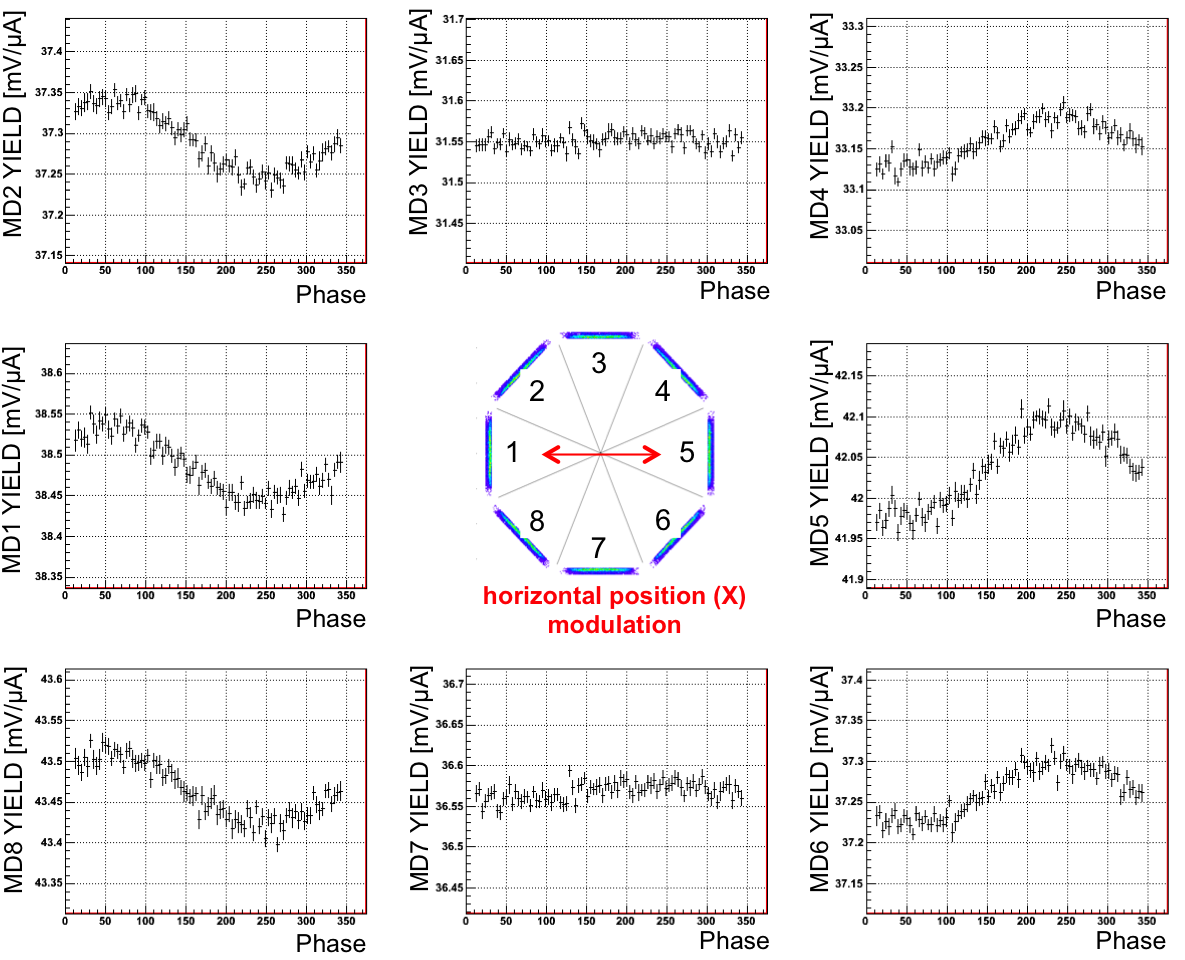
\includegraphics[width=15.0cm]{figures/BModDetectorResponse}
%	\end{center}
%	\caption{Target BPM Detector to X Position Modulation. }
%	\label{fig:BModDetectorResponse}
%\end{figure}
%\end{singlespace}

\begin{singlespace}
\begin{figure}[!h]
	\begin{center}
	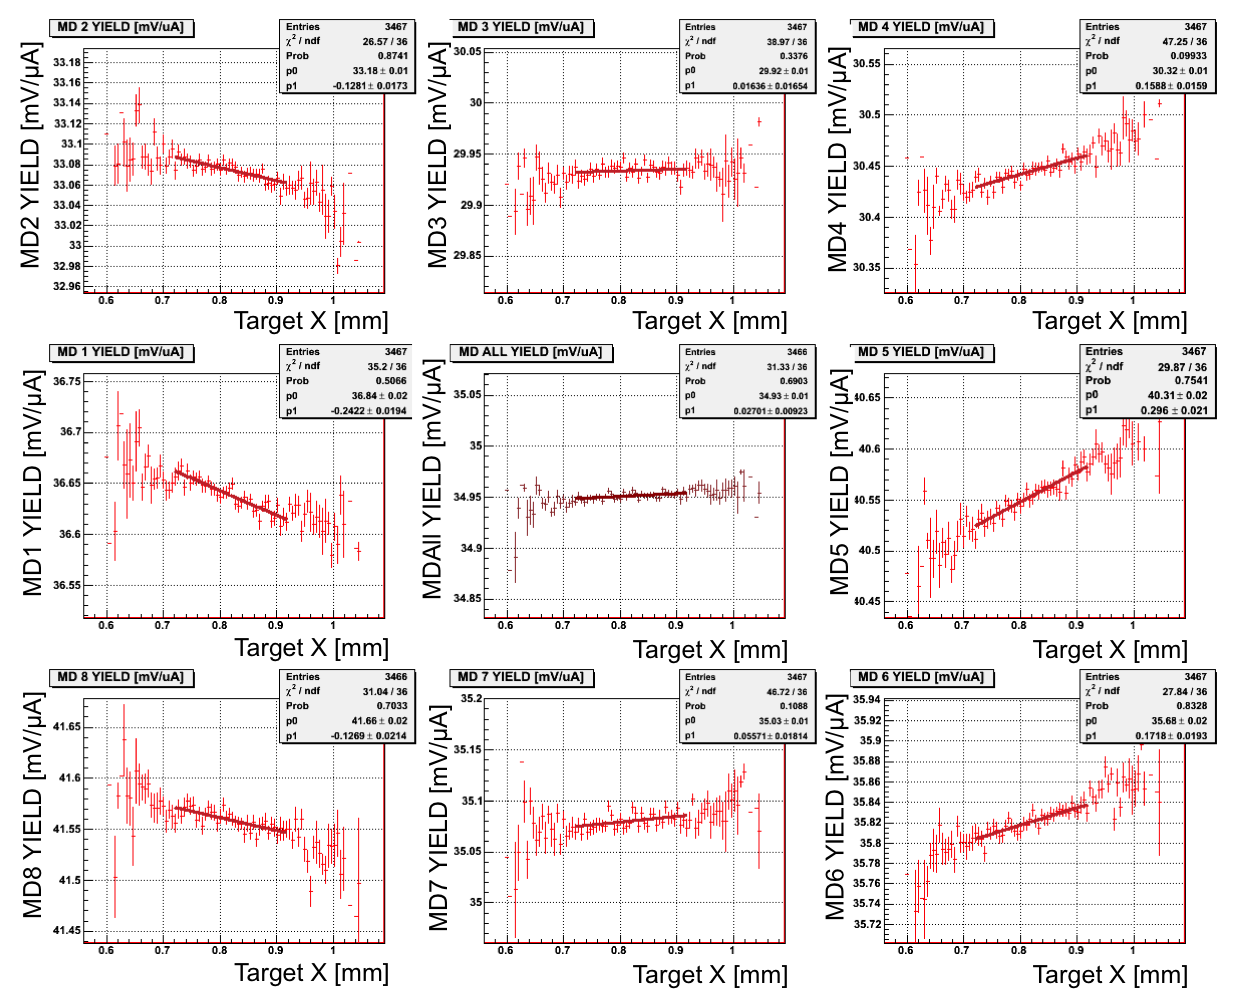
\includegraphics[width=15.0cm]{figures/BModDetectorSensitivity}
	\end{center}
	\caption
%	[Main detector sensitivities with respect to target BPM X position for X Position Modulation.]	
	{Main detector sensitivities with respect to target BPM X position for X Position Modulation.}
	\label{fig:BModDetectorSensitivity}
\end{figure}
\end{singlespace}

A typical detector sensitivity for X modulation during an hour long run is shown in Figure~\ref{fig:BModDetectorSensitivity}. The detector sensitivities for all beam parameters for a few days during Run 1 are shown in Figure~\ref{fig:BModSensitivities}. 
Beam modulation amplitudes at the target, as well as typical monthly results measured for the HC beam properties $\Delta T_{i}$ and detector sensitivities $\partial A /\partial T_{i}$ during Run 2 can be found in Table~\ref{tab:bmod_sensitivities}. The HC beam asymmetries for X, X$^\prime$ are anti-correlated and largely cancel. The same is true for Y and Y$^\prime$. The uncertainties associated with the monthly HC position (angle) differences $\Delta T_{i}$ are 0.07~nm (0.01~nrad) based on the quartet level BPM resolution (discussed in section~\ref{BPM Resolution}), shown in Table~\ref{tab:bmod_sensitivities}. 

\begin{singlespace}
\begin{figure}[!h]
	\begin{center}
	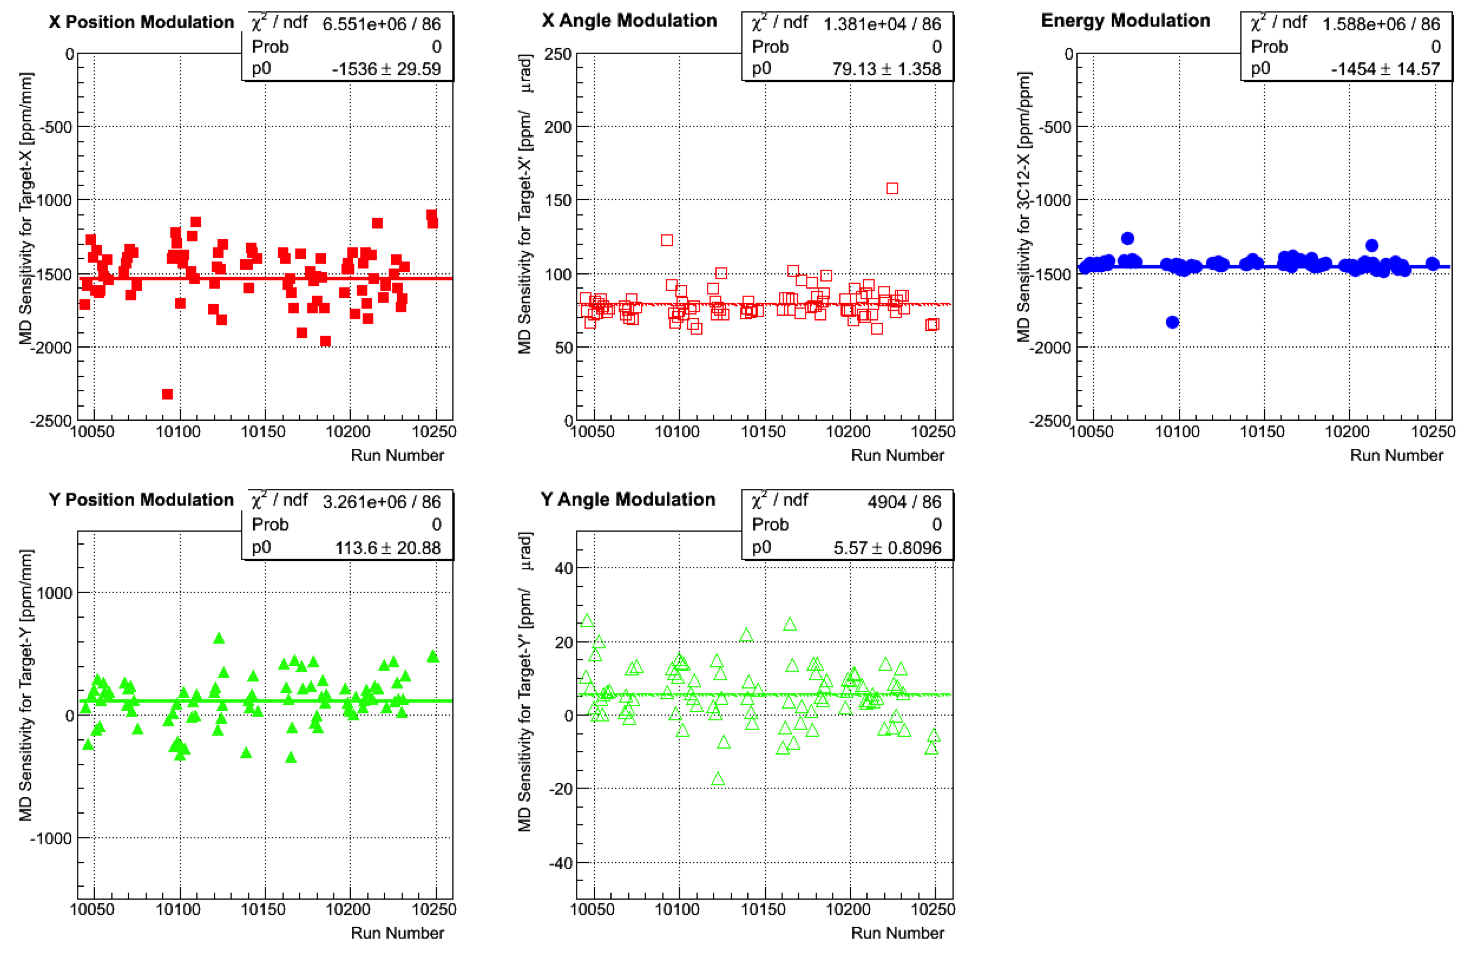
\includegraphics[width=15.0cm]{figures/BModSensitivities}
	\end{center}
	\caption
%	[Main detector sensitivities for X, X$^\prime$, E, Y, and Y$^\prime$.]
	{Main detector sensitivities for X (solid red square), X$^\prime$ (empty red square), E (solid blue square), Y (solid green triangle), and Y$^\prime$ (empty green triangle) are shown. }
	\label{fig:BModSensitivities}
\end{figure}
\end{singlespace}


\begin{singlespace}
\begin{table}[!h]
\begin{center}
  	\caption
%	[A typical amplitudes used for driven beam modulation. BPM differences and sensitivities during Run 2.]
  	{A typical amplitudes used for driven beam modulation (column 2). Columns 3 and 4 provide typical average monthly results measured during Run 2 for the helicity correlated beam parameter differences $\Delta T_{i}$ and detector sensitivities $\partial{A}/\partial{T_{i}}$ for the beam parameters i listed in the first column. The total HCBA for this example is only 0.4~ppb. The uncertainties associated with $\Delta T_{i}$  and $\partial A /\partial T_{i}$ are discussed in the text~\cite{Allison:2014tpu}.}
  \begin{tabular}{ c | c | c | c }
%    \hline
    \noalign{\hrule height 1pt}
    Beam  		& Modulation	& Differences 	& Sensitivities 	\\
    Parameter	& Amplitude 	& [monthly] 		& [monthly] 		\\ 
%    \hline
    \noalign{\hrule height 1pt}
    X 						& $\pm$125~$\mu$m	& -3.3~nm & -2.11~ppm/$\mu$m \\
    Y 						& $\pm$125~$\mu$m 	& 2.5~nm & 0.24~ppm/$\mu$m \\
    X$^{\prime}$	& $\pm$5~$\mu$rad 		& -0.7~nrad & 100.2~ppm/$\mu$rad \\
    Y$^{\prime}$	& $\pm$5~$\mu$rad 		& 0.002~nrad & -0.0~ppm/$\mu$rad \\
    E 						& $\pm$61~ppm (70~keV) 	& 0.1~nm & -1.56~ppm/$\mu$m \\
%    \hline
    \noalign{\hrule height 1pt}
  	\end{tabular}
  \label{tab:bmod_sensitivities}
\end{center}
\end{table}
\end{singlespace}

A subset of the Run 2 parity violating electron-proton scattering production data showing the blinded asymmetry grouped by (monthly) Wien state is shown in Figure~\ref{fig:BModNaturalCorrections}~\cite{Allison:2014tpu}. Two different approaches to determine the sensitivities of the apparatus to HC beam properties were used to correct for the false asymmetry. The measured asymmetries without any correction (solid squares) are compared to the asymmetries after correction using the intrinsic random variations in beam properties (natural motion: triangles) and to the asymmetries using the beam modulation (beam modulation: inverted triangles). The asymmetries derived using each techniques are consistent with each other, and the overall correction for HC beam asymmetries is small. The data shown here represent 80\% of the Run 2 data for which modulation was available. %Run 1 provides an additional 1/3 of the total data acquired in the experiment~\cite{Allison:2014tpu}. 
An additional 1/3 of the total data acquired in the experiment was provided by Run 1 dataset. 
%More updated analysis on modulation sensitivities can be found in future theses of J. Hoskins~\cite{jhoskins_thesis} and D. Jones~\cite{don_thesis}
More detailed description of modulation sensitivity analysis and recent results will be discussed by J. Hoskins~\cite{jhoskins_thesis} and D. Jones~\cite{don_thesis} in their future theses.

\begin{singlespace}
\begin{figure}[!h]
	\begin{center}
	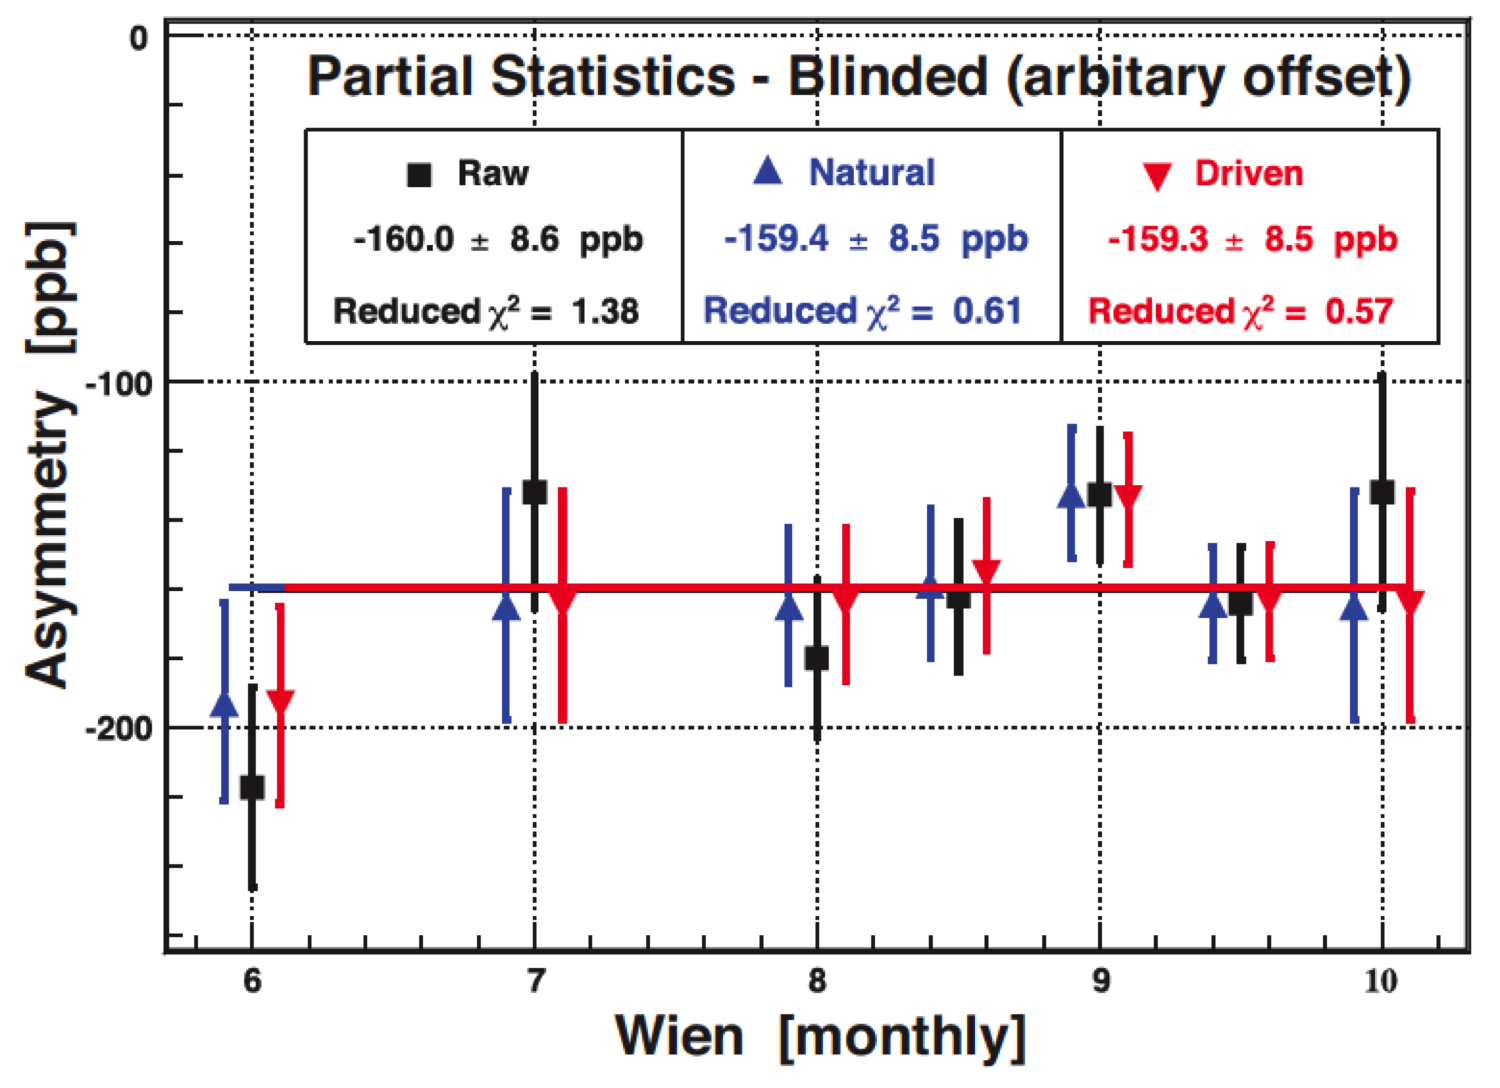
\includegraphics[width=12.0cm]{figures/BModNaturalCorrections}
	\end{center}
	\caption
%	[Corrected asymmetry using BMod and natural motion grouped by Wien.]
	{Subset of the Run 2 production data showing the blinded asymmetry (in ppb) grouped by (monthly) Wien state, and corrected using two different approaches to determine the sensitivities of the apparatus to HC beam properties that can give rise to false asymmetries. Other needed corrections are not applied to the data in this figure. The results without any correction (solid squares) are compared to the results after correction using the intrinsic random variations in beam properties (Natural motion: upward pointing triangles) and to the results using the driven beam motion (Beam modulation: downward pointing triangles) where the sensitivities are derived by actively modulating each property of the beam with a magnitude significantly larger than that intrinsically carried by the beam. The asymmetries derived using each technique are consistent with each other, and the overall correction for HCBAs is small. The data shown here represent the 80\% of the Run 2 data for which driven motion was available. Run 1 provides an additional $\sim$1/3 of the total data acquired in the experiment~\cite{Allison:2014tpu}.}
	\label{fig:BModNaturalCorrections}
\end{figure}
\end{singlespace}



%Regression uses a linear regression algorithm that minimizes the correlation of
%the detector responses to the “natural” beam motion inferred from the responses of
%the beam monitors, and corrects Araw for AFb. Regression corrections to Araw are
%discussed in Section 7.3.2.2. - Rupesh 





%%%%%%%%%%%%%%%%%%%%%%%%%%%%%%%%%%%%%%%%%%%%%%%%%%%%%%%%%%%%%
\section{Beamline Optics}
\label{Beamline Optics}
%The experiment was performed at the Thomas Jefferson National Accelerator Facility (Jefferson Lab) in Newport News, Virginia. The electron accelerator is known as Continuous Electron Beam Accelerator Facility (CEBAF) and is capable of probing nucleon and quark structure in nuclei\cite{sarah_G0}.
A typical BPM response to modulation drive signal is sinusoidal and is shown in Figure~\ref{fig:BModBPMResponse} in the previous chapter. The responses from all 23\footnote{There were 24 BPMs in the Hall-C beamline. BPM 3H09B died after Run 1, hence excluded from the analysis.} BPMs in the Hall-C beamline to modulation signal were observed throughout the production data collection. The BPM responses in X due to X modulation are shown in Figure~\ref{fig:BModBpmsX}. The vertical axis is the BPM X-signal for X kick and the horizontal axis is the phase (the ramp-wave was used to monitor the phase of the drive signals). The data are shown in red and fits are in dark red. The BPM responses are arranged according to the distance from the target. 
Beam position response amplitudes of all the BPMs to X modulation (from Figure~\ref{fig:BModBpmsX}) with respect to Z locations from the target are shown in Figure~\ref{fig:BModOpticsX}. 
The location of all the BPMs are shown at the top of the plot by short vertical lines. All the quadrupoles, dipoles, Compton dipoles, M{\o}ller magnets, target, and beam modulation magnets are shown by short vertical lines at the bottom. Data are shown in solid circles, and simulated points from OptiM are shown in empty squares. This figure represents the evolution of the position response amplitude to modulation drive signal along the Hall-C beamline. The data matches quite well with the simulation. This method of tracking BPM response also helped to find any optics change or hardware failure in the beamline. 

%\begin{singlespace}
%\begin{figure}[!h]
%	\begin{center}
%	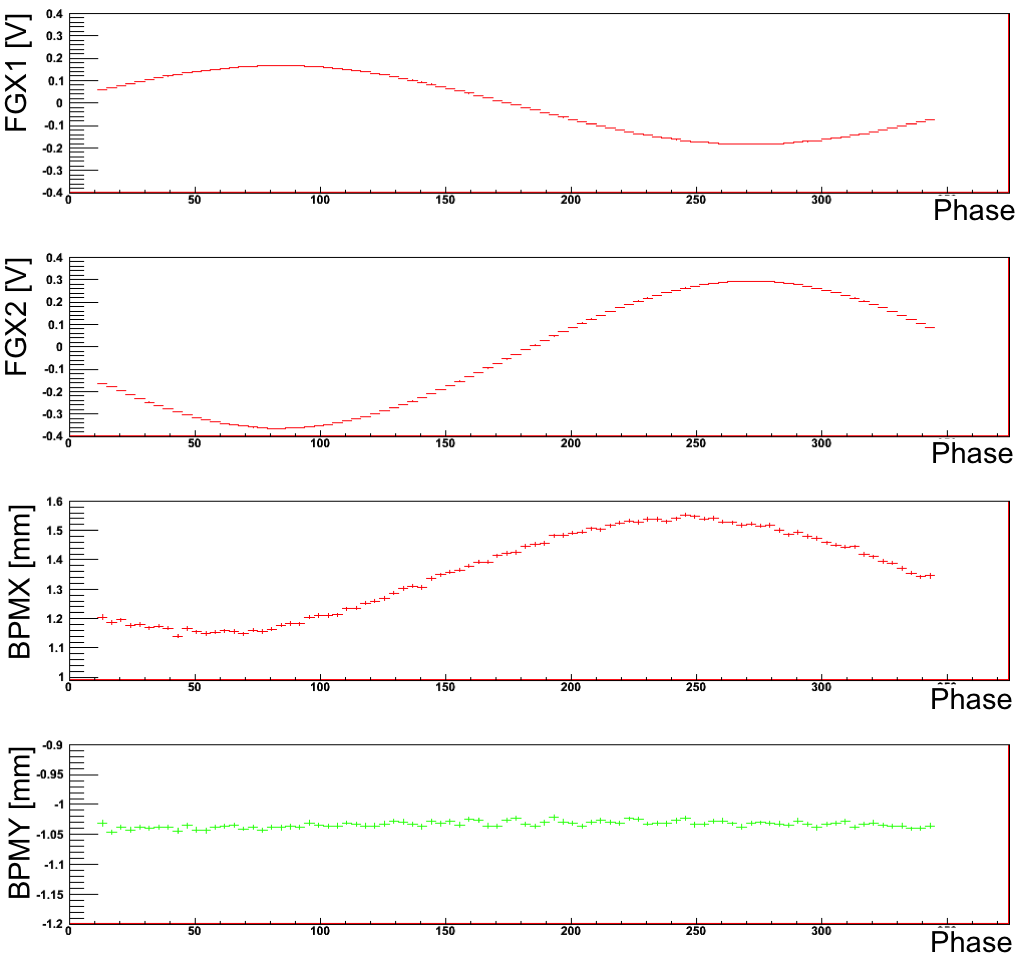
\includegraphics[width=10.0cm]{figures/BModBPMResponse}
%	\end{center}
%	\caption{Target BPM Response to X Position Modulation. }
%	\label{fig:BModBPMResponse}
%\end{figure}
%\end{singlespace}


\begin{singlespace}
\begin{figure}[!h]
	\begin{center}
	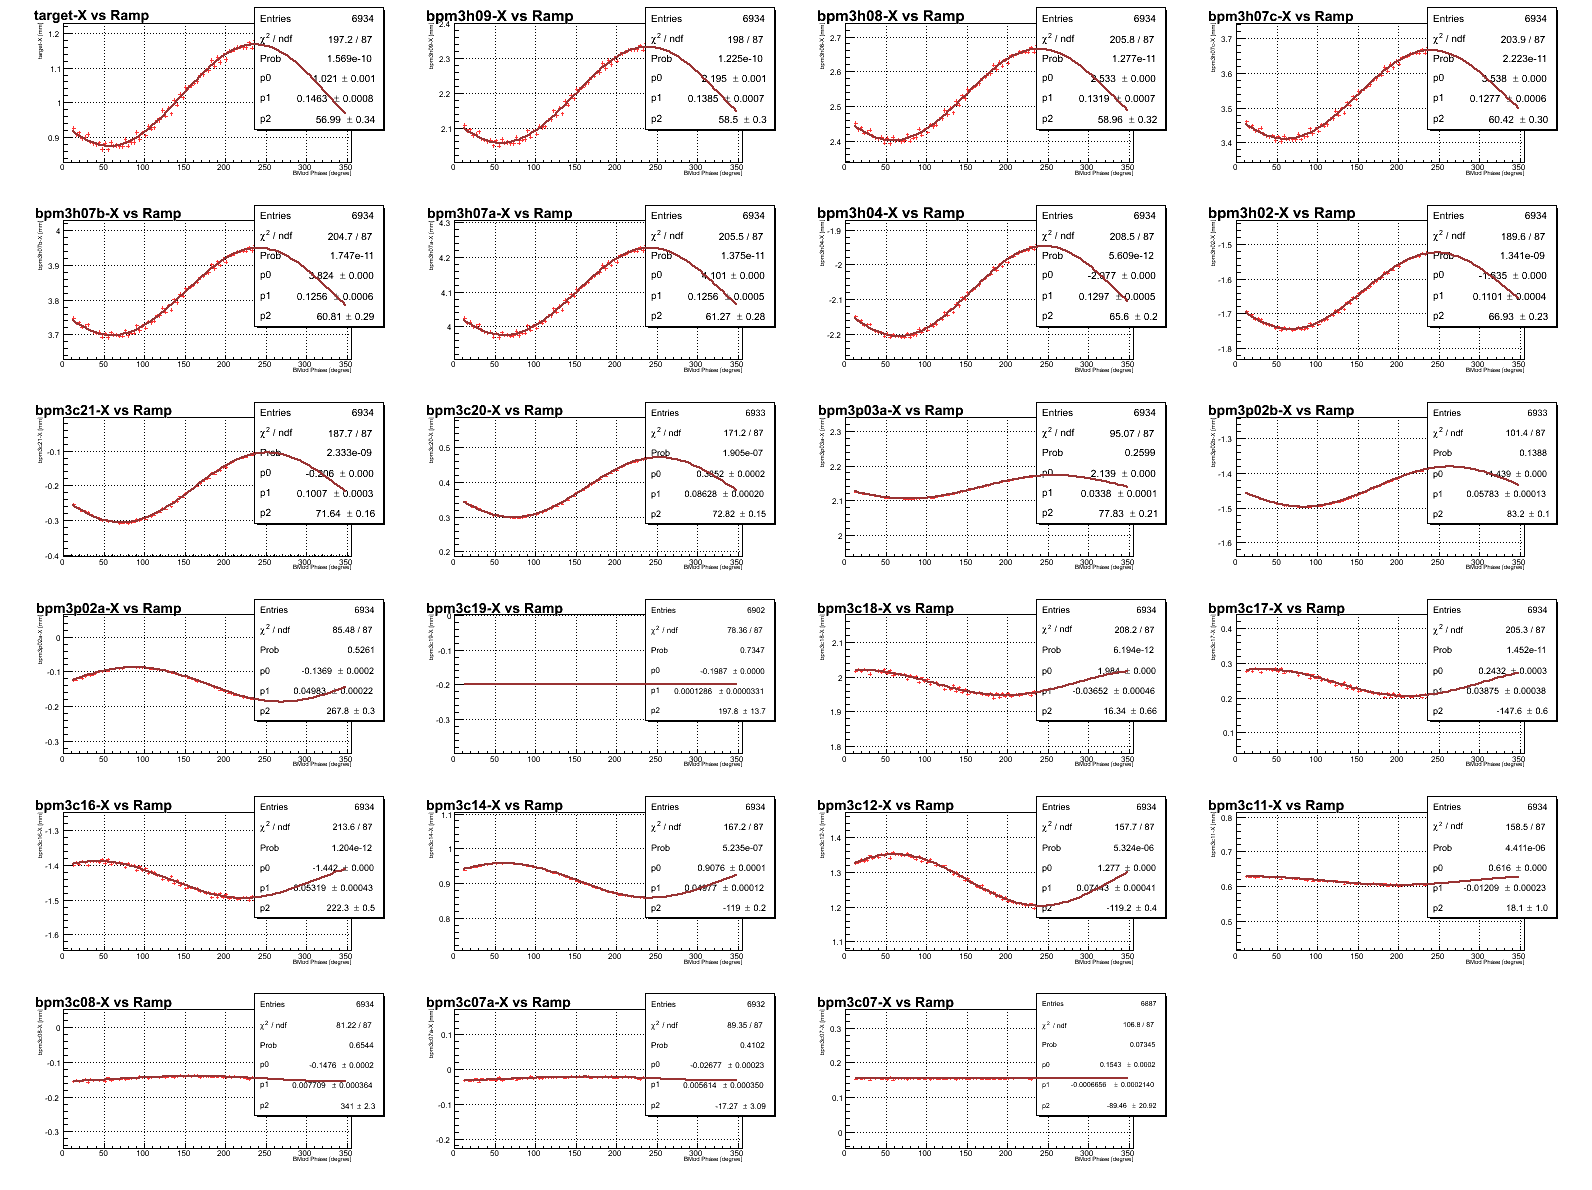
\includegraphics[width=15.0cm]{figures/BModBpmsX}
	\end{center}
	\caption
%	[All Hall-C BPM responses in X due to X modulation using a pair of coils.]
	{All Hall-C BPM responses in X due to X modulation using a pair of coils. The vertical axis is BPM X-response and horizontal axis is ramp-wave (the ramp-wave was used to monitor the phase of the drive signals). The data are shown in red and fits are shown in dark red. Starting at the target BPM in the top left, upstream BPMs are shown along the left to right and top to bottom directions, BPM 3C07 being the first BPM in the Hall-C beamline. 
	}
	\label{fig:BModBpmsX}
\end{figure}
\end{singlespace}


\begin{singlespace}
\begin{figure}[!h]
	\begin{center}
	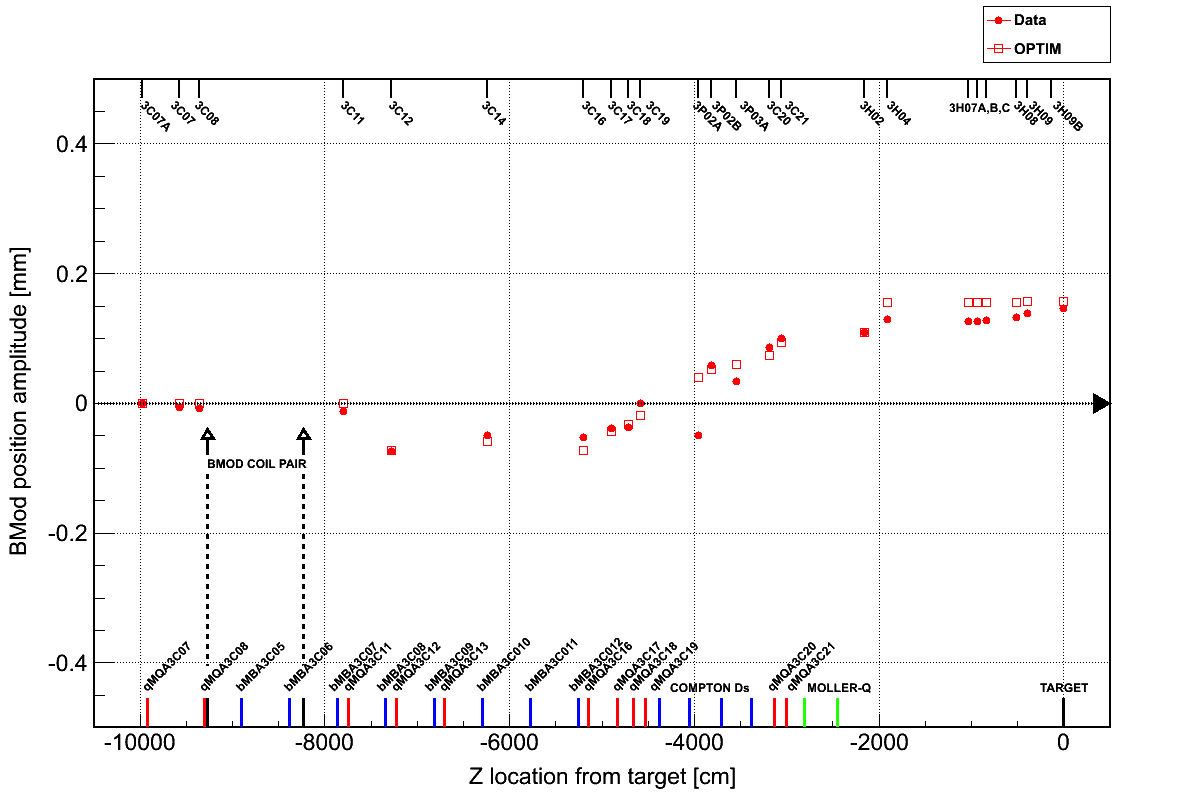
\includegraphics[width=15.0cm]{figures/BModOpticsX}
	\end{center}
	\caption
%	[Beam position response of all the BPMs in the Hall-C beamline to X modulation.]	
	{Beam position response of all the BPMs in the Hall-C beamline to X modulation. The locations of all the BPMs are shown at the top of the plot by vertical line. All the quadrupoles, dipoles, Compton dipoles, M{\o}ller magnets, target, and BMod magnets are shown at the bottom of the plot by vertical lines. Data are shown in solid circles, and simulated points from OptiM are shown in empty squares.}
	\label{fig:BModOpticsX}
\end{figure}
\end{singlespace}



\begin{singlespace}
\begin{figure}[!h]
	\begin{center}
	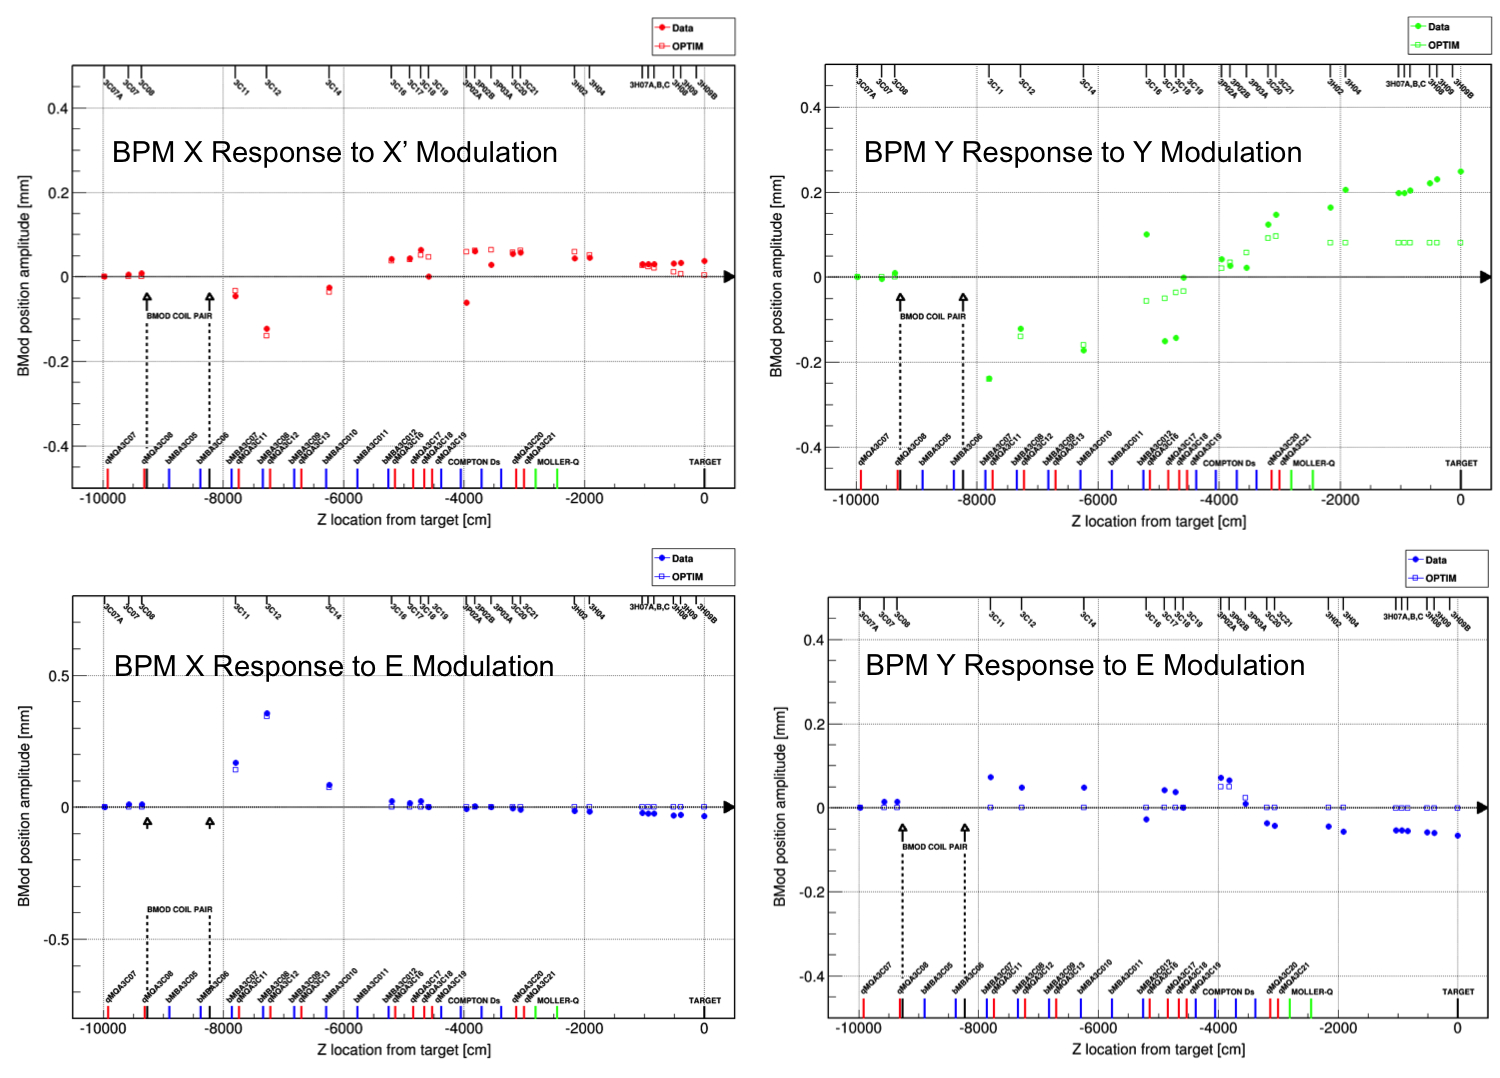
\includegraphics[width=15.0cm]{figures/BModOpticsMISC}
	\end{center}
	\caption
%	[Beam position response of all the BPMs in the Hall-C beamline to X modulation.]
	{Beam position response of all the BPMs in the Hall-C beamline to X modulation. The locations of all the BPMs are shown at the top of the plot by vertical line. All the quadrupoles, dipoles, Compton dipoles, M{\o}ller magnets, target, and BMod magnets are shown at the bottom of the plot by vertical lines. Data are shown in solid circles, and simulated points from OptiM are shown in empty squares.}
	\label{fig:BModOpticsMISC}
\end{figure}
\end{singlespace}


The BPM responses in $X$ due to $X^{\prime}$ modulation, responses in $Y$ due to $Y$ modulation, responses in $Y$ due to $E$ modulation, and responses in $X$ due to $E$ modulation are shown in Figure~\ref{fig:BModOpticsMISC} (from top left along the clockwise direction). 
The Fast Feed Back (FFB) system was fighting with the modulation system which is more evident in the $X^{\prime}$ modulation response (see section~\ref{Effect of Fast Feed Back on Beam Modulation} for more details). There was a defocus in $Y$ modulation and the system was not able to achieve a relatively pure $Y$ position at the target. The residual dispersion at the target X was evident from the $E$ modulation and was as high as $\sim$1/7th of the dispersion of the middle of the arc. The residual dispersion in Y was also non-negligible.
These responses were recorded for all the production runs. The target BPM and BPM 3C12 position responses to X modulation vs. time for Run 1 and Run 2 are shown in Figure~\ref{fig:BMod_XMod_Xresponse}. The target X position was unstable at the beginning of the experiment. The big dip in the amplitude around run number 10900 was due to change in ``tune" (BMod magnet current ratio) in order to achieve a better decoupling in the beam parameters. The optics was very stable from run number 11900 onward. There was a constant residual dispersion at the target throughout the experiment.



\begin{singlespace}
\begin{figure}[!h]
	\begin{center}
	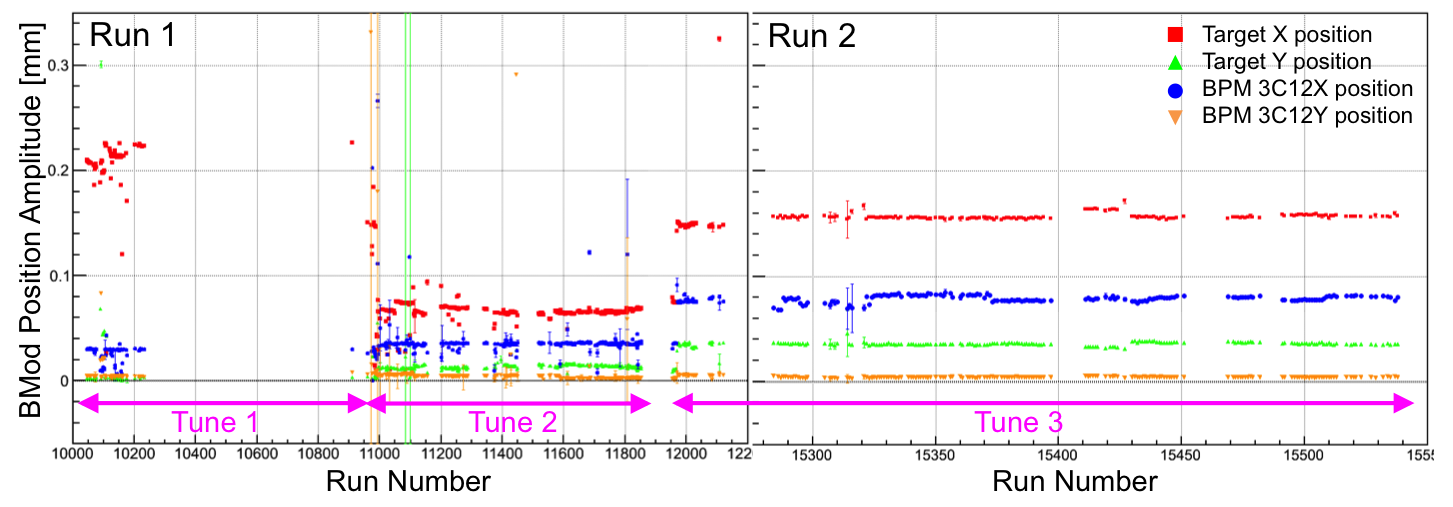
\includegraphics[width=15.0cm]{figures/BMod_XMod_Xresponse}
	\end{center}
	\caption
%	[Hall-C target BPM responses due to modulation kick using a pair of coil in X.]	
	{
%	Beam position response of all the BPMs in the Hall-C beamline to X modulation. The location of all the BPMs are shown at the top of the plot by vertical line. All the quadrupoles, dipoles, Compton dipoles, M{\footnotesize$\varnothing$}ller magnets, target, and BMod magnets are shown at the bottom of the plot by vertical lines. Data are shown in solid circle, and simulated points from OptiM are shown in empty square.
Hall-C target BPM responses due to modulation kick using a pair of coils in X. The sinusoidal response of the target BPM of a modulation signal for relatively pure X is fitted and the amplitude of the sinusoidal signal is plotted in vertical axis. The vertical axis is BMod BPM position in mm. The X target position is shown with solid red diamond, Y target position is shown with solid green triangle, BPM 3C12 X position is shown with solid blue square, BPM 3C12 Y position is shown with solid orange circle. For a relatively pure X position motion, we expect largely X target response and very small X angle response. We do not expect any Y position or Y angle response in this case. BPM 3C12X position response is relatively constant and 3C12Y is consistent with zero.		
	 }
	\label{fig:BMod_XMod_Xresponse}
\end{figure}
\end{singlespace}


%\begin{singlespace}
%\begin{figure}[!h]
%	\begin{center}
%	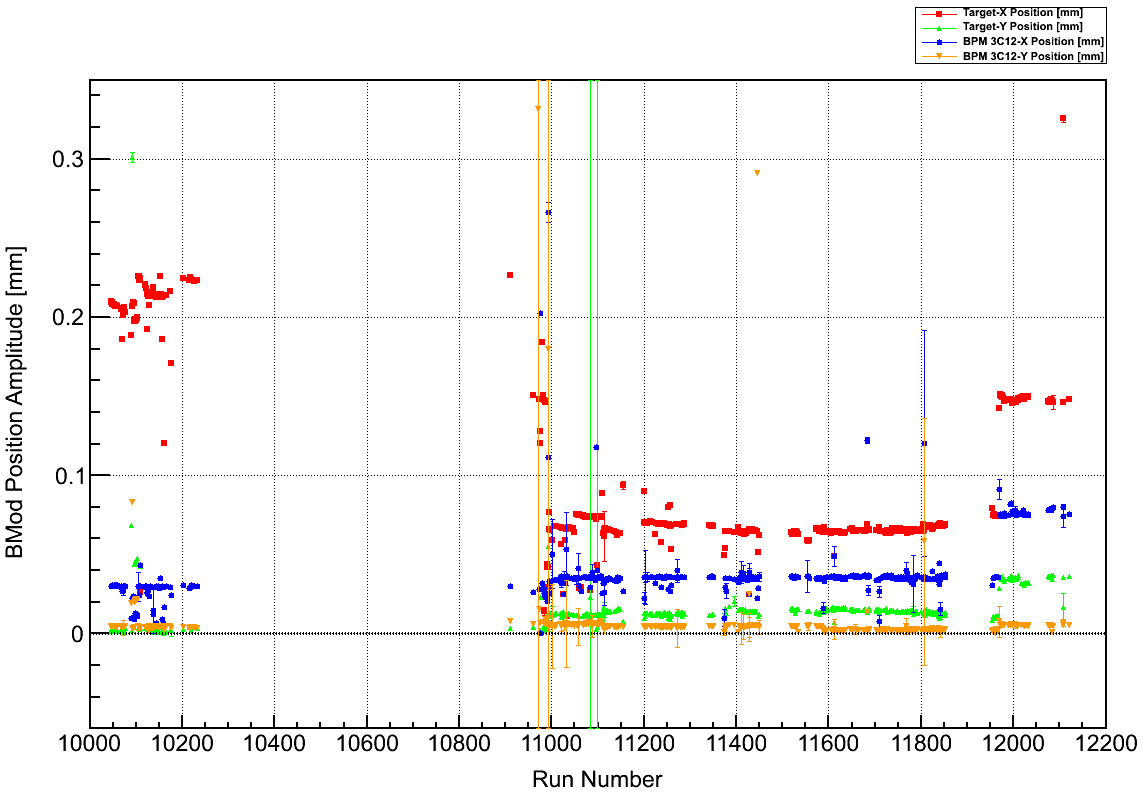
\includegraphics[width=15.0cm]{figures/run1_XMod_Xresponse}
%	\end{center}
%	\caption{
%%	Beam position response of all the BPMs in the Hall-C beamline to X modulation. The location of all the BPMs are shown at the top of the plot by vertical line. All the quadrupoles, dipoles, Compton dipoles, M{\footnotesize$\varnothing$}ller magnets, target, and BMod magnets are shown at the bottom of the plot by vertical lines. Data are shown in solid circle, and simulated points from OptiM are shown in empty square.
%Hall-C target BPM responses due to modulation kick using a pair of coil in X. The sinusoidal response of the target BPM of a modulation signal for relatively pure X is fitted and the amplitude of the sinusoidal signal is plotted in vertical axis. The vertical axis is BMod BPM position in cm. The X target position is shown with solid red diamond, Y target position is shown with solid green triangle, BPM 3C12 X position is shown with solid blue square, BPM 3C12 Y position is shown with solid orange circle. For a relatively pure X position motion, we expect largely X target response and very small X angle response. We don’t expect any Y position or Y angle response in this case. BPM 3C12X position response is relatively constant and 3C12Y is consistent
%with zero.		
%	 }
%	\label{fig:run1_XMod_Xresponse}
%\end{figure}
%\end{singlespace}
%
%\begin{singlespace}
%\begin{figure}[!h]
%	\begin{center}
%	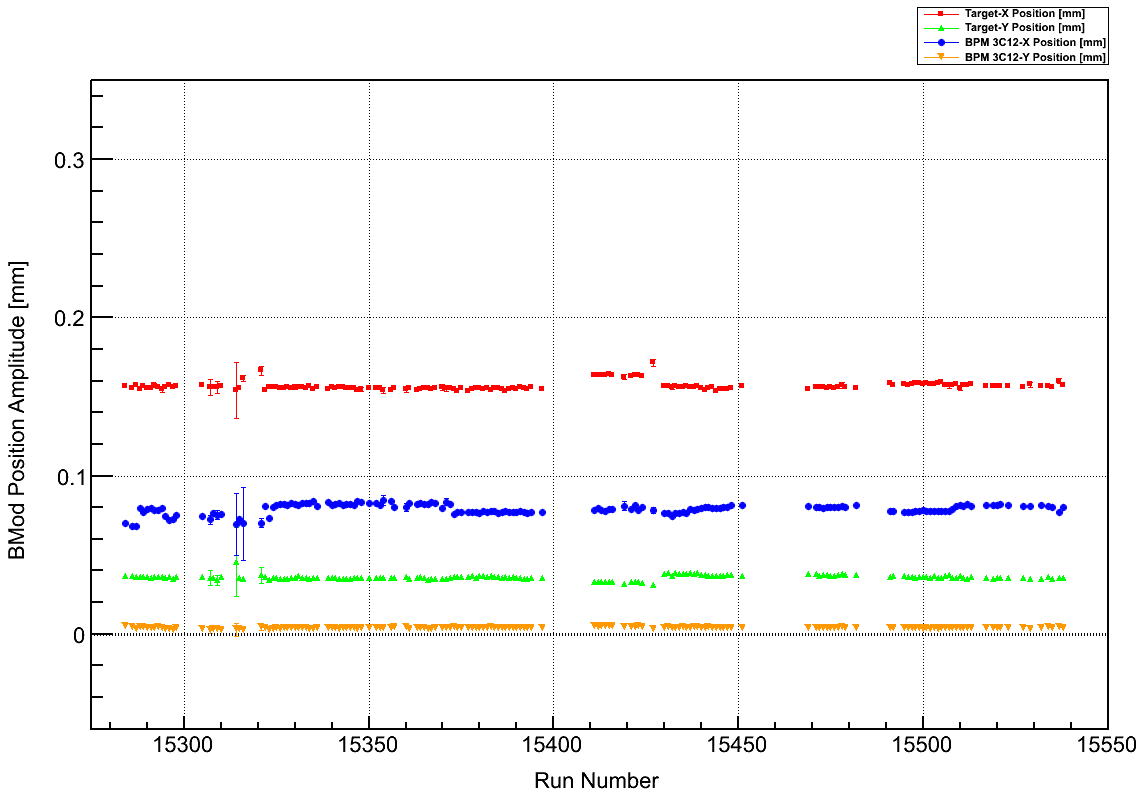
\includegraphics[width=15.0cm]{figures/run2_XMod_Xresponse}
%	\end{center}
%	\caption{Beam position response of all the BPMs in the Hall-C beamline to X modulation. The location of all the BPMs are shown at the top of the plot by vertical line. All the quadrupoles, dipoles, Compton dipoles, M{\footnotesize$\varnothing$}ller magnets, target, and BMod magnets are shown at the bottom of the plot by vertical lines. Data are shown in solid circle, and simulated points from OptiM are shown in empty square. }
%	\label{fig:run2_XMod_Xresponse}
%\end{figure}
%\end{singlespace}
%


\begin{singlespace}
\begin{figure}[!h]
	\begin{center}
	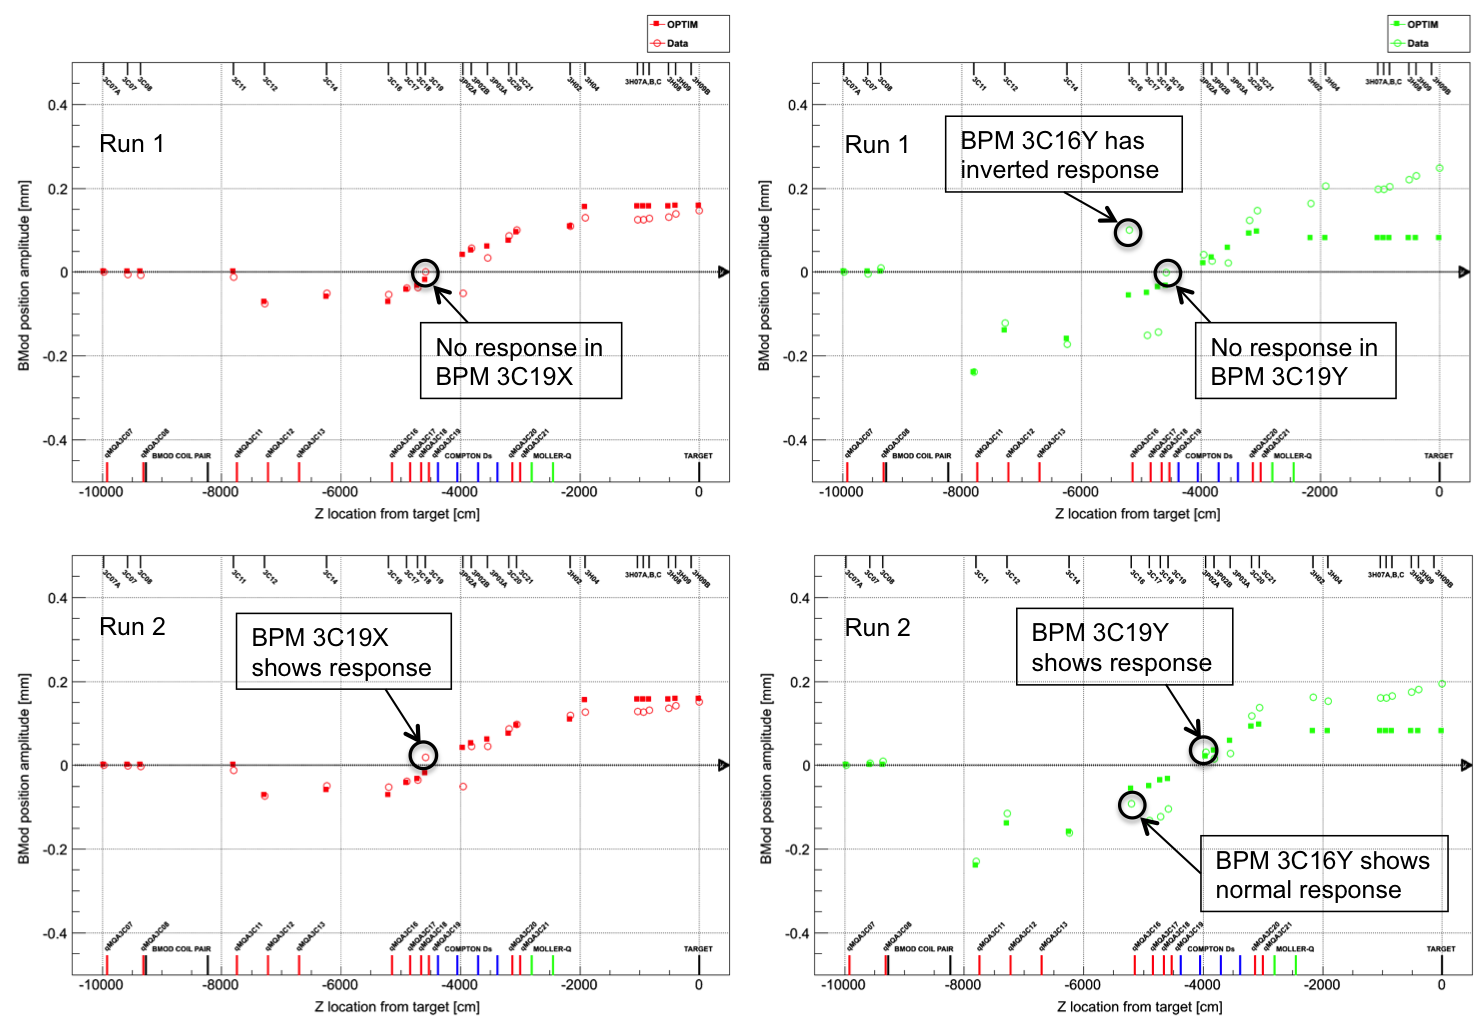
\includegraphics[width=15.0cm]{figures/BModBPMSignCorrection}
	\end{center}
	\caption
%	[The beam position response of all the BPMs in the Hall-C beamline to X modulation.]
	{The beam position response of all the BPMs in the Hall-C beamline to X modulation. The locations of all the BPMs are shown at the top of the plot by vertical line. All the quadrupoles, dipoles, Compton dipoles, M{\o}ller magnets, target, and BMod magnets are shown at the bottom of the plot by vertical lines. Data are shown in solid circles, and simulated points from OptiM are shown in empty squares.}
	\label{fig:BModBPMSignCorrection}
\end{figure}
\end{singlespace}


\subsection{BPM Sign Corrections}
\label{BPM Sign Corrections}

The beam modulation system also helped to track some of the problems in the BPMs in the Hall-C beamline. During Run 1, BPM 3C19X (as shown in Figure~\ref{fig:BModBPMSignCorrection}) and Y showed no response to any modulation drive signals, whereas BPM 3C16Y showed an inverted response (more details in APPENDIX~\ref{Beam Modulation 2}). After investigation, misconnected cables were found for those BPMs and repaired before Run 2. 
Another problem was found with the BPMs 3P02A and 3P02B in the Compton region. These Compton BPMs had a different rotation in the beamline compared to the all other BPMs, hence they responded differently to the modulation signal. This problem was fixed in the software by giving an offset angle for these BPMs.
The BPMs discussed above did not affect any physics results for Run 1, as they were not used in any asymmetry or regression calculation. 

%Motivation:
%During Run 1, BPM 3C19X and Y showed zero response to different modulation signal. BPM 3C16Y showed inverted response to modulation signals.
%
%Figure 1 and 2 is for run 12000 from 7th May 2011. This is a typical production run from Run 1 and also represent it. Here in Figure 1 we observed BPM 3C19X has zero response to X-modulation. In Figure 2 we observed BPM 3C19Y has zero and 3C16Y has inverted response to Y-modulation.
%
%Figure 3 and 4 is for run 15646 from 31st January 2012. This is a production run. In Figure 3 we observed a non zero BPM 3C19X response to X-modulation. In Figure 4 we observed BPM 3C19Y has non zero and 3C16Y has inverted response to Y-modulation.
%
%Figure 5 and 6 is for run 15646 from 2nd February 2012. This is a production run. In Figure 5 we observed a non zero BPM 3C19X response to X-modulation. In Figure 6 we observed BPM 3C19Y has non zero and 3C16Y has normal response to Y-modulation.
%
%Summary:
%After cable swapping in BSY on 2nd January and 1st February 2012 the BPM 3C19 and 3C16 seems to be working fine.

%\subsection{Effect of Beam Modulation System on Production Data}
%\label{Effect of Beam Modulation System on Production Data}

\subsection{Beam Modulation Tune Parameter Scan}
\label{Beam Modulation Tune Parameter Scan}

The idea of this analysis was to find a relatively pure angle and position ``tune" at the target for the modulation system. In order to achieve a pure X and Y position and angle at the target, scan of the ``tune" parameters was performed by varying the ratio of the drive signals in small steps. The maximum amplitudes of the function generator drive signals for this test were set to 0.444 times of the nominal amplitudes (shown in Table~\ref{tab:beam_parameter}, chapter~\ref{BEAM MODULATION}) for caution. The tune parameters were changed by changing the current in one coil ($I_{1}$) in steps of 50\%, 25\%, 0\%, -25\%, and -50\%, respectively keeping the other coil ($I_{2}$) fixed to achieve a ``tune" that generates a relatively pure angle at the target. 
A relatively pure X-angle tune was found to be in between the tune parameters -5.882 (nominal) and -9.009 (53.2\%), and Y-angle to be in between -0.500 (nominal) and -0.675 (35\%). The ``tunes" for X and Y positions were already good to produce relatively pure position at the target. Based on this analysis, the modulation ``tunes" were changed during Run 1 and are shown in Figure~\ref{fig:BMod_XMod_Xresponse}.


%Figure 1: Hall-C BPM responses in X due to kick using a pair of coil in X angle. The vertical axis is BPM X-signal amplitude and horizontal axis is beamline elements. OptiM simulation predicted points are shown in solid red square and data is shown in empty red circle. We changed the tune parameters (ratio of currents in the magnets) by 100\%, 53.2\%, 0\%, -25.8\% and -33.3\% by changing the current in one coil(I1) in steps of 50\%, 25\%, 0\%, -25\% and -50\% respectively keeping the other coil(I2) fixed to achieve a tune that generates pure angle at the target. Previously we didn't achieved a pure X angle at target with our nominal tune(See ELOG: https://qweak.jlab.org/elog/Beam/95). Form the results it appears that a pure X- angle tune exist in between the tune parameters -5.8824(0\%) and -9.0090(53.2\%). See details in Table 1 of attachment 5.
%
%Figure 2: Hall-C BPM responses in Y due to kick using a pair of coil in Y angle. The vertical axis is BPM Y-signal amplitude and horizontal axis is beamline elements. OptiM simulation predicted points are shown in solid green square and data is shown in empty green circle. We changed the tune parameters by -50\%, -25\%, 0\%, 25\% and 50\% by changing the current in one coil(I2) in steps of -50\%, -25\%, 0\%, 25\% and 50\% respectively keeping the other coil(I1) fixed to achieve a tune that generates pure angle at the target. Previously we didn't  achieved a pure Y angle at target with our nominal tune(See ELOG: https://qweak.jlab.org/elog/Beam/95). Form the results it appears that a pure Y- angle tune exist in between the tune parameters -0.500(0\%) and -0.675(35\%). See details in Table 2 of attachment 5.
%
%Figure 3: Hall-C BPM responses in X due to kick using a pair of coil in X. The vertical axis is BPM X-signal amplitude and horizontal axis is beamline elements. OptiM simulation predicted points are shown in solid red square and data is shown in empty red circle. We were already happy with X (See ELOG: https://qweak.jlab.org/elog/Beam/95). We changed the tune parameters by -9.1\%, -4.6\%, 0\%, 5.5\%, 11.1\% by changing the current in one coil(I1) in steps of 10\%, 5\%, 0\%, -5\% and -10\% respectively keeping the other coil(I2) fixed. See details in Table 3 of attachment 5.
%
%Figure 4: Hall-C BPM responses in Y due to kick using a pair of coil in Y. The vertical axis is BPM Y-signal amplitude and horizontal axis is beamline elements. OptiM simulation predicted points are shown in solid green square and data is shown in empty green circle. For this case it was giving us almost a pure position in Y and we were happy with it (See ELOG: https://qweak.jlab.org/elog/Beam/95). We changed the tune parameters  by 10\%, 4.9\%, 0\%, -5.1\%, 10\% by changing the current in one coil(I2) in steps of 10\%, 5\%, 0\%, -5\% and -10\% respectively keeping the other coil(I1) fixed. See details in Table 4 of attachment 5.


\begin{singlespace}
\begin{figure}[!h]
	\begin{center}
	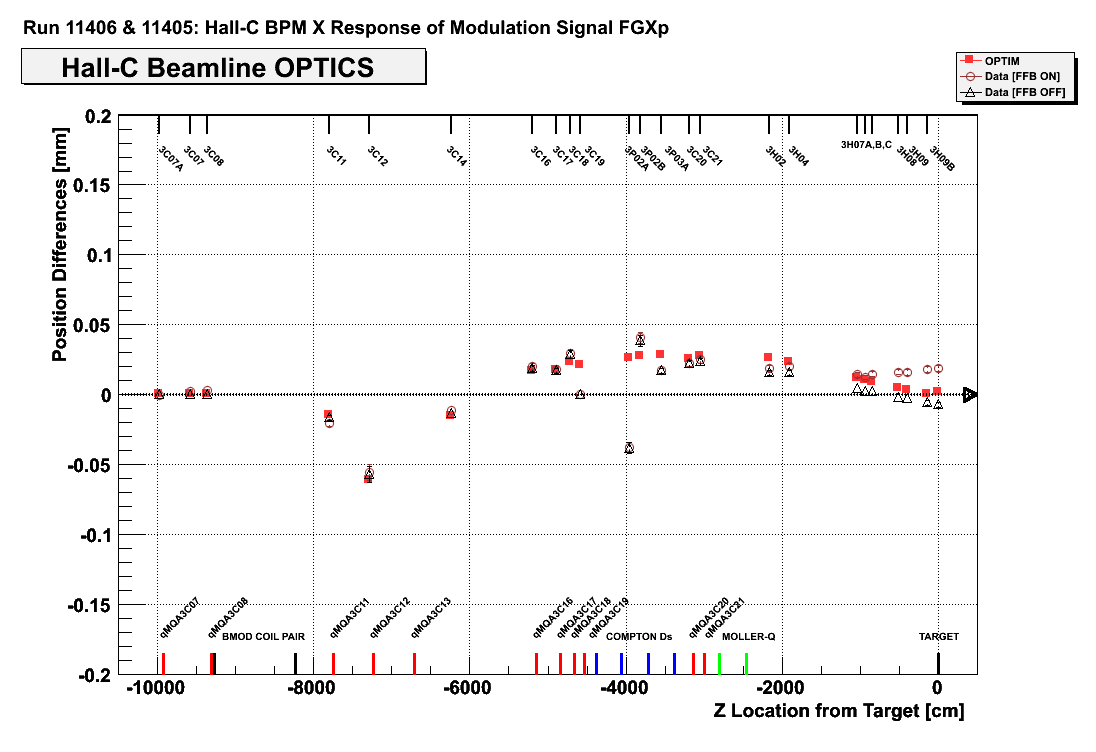
\includegraphics[width=15.0cm]{figures/BModOpticsFFBXXp}
	\end{center}
	\caption
%	[Hall-C BPM responses in X due to X angle modulation using a pair of coils.]
	{Hall-C BPM responses in X due to X angle modulation using a pair of coils. The vertical axis is BPM X-signal amplitude and horizontal axis is beamline elements. The simulated points from OptiM are shown in solid red squares, data with FFB ON are shown in empty red circles and data with FFB OFF are shown in empty black triangles. There is almost no effect of FFB on data for X motion. The locations of all the BPMs are shown at the top of the plot by vertical lines. All the quadrupoles, dipoles, Compton dipoles, M{\o}ller magnets, target, and BMod magnets are shown at the bottom of the plot by vertical lines. }
	\label{fig:BModOpticsFFBXXp}
\end{figure}
\end{singlespace}

\subsection{Effect of Fast Feed Back on Beam Modulation\index{FFB!Effect on Beam Modulation}}
\label{Effect of Fast Feed Back on Beam Modulation}

%The idea of this analysis was to show the effect of the Fast Feed Back (FFB) on the beam modulation system. 
The Fast Feed Back (FFB) system was designed to suppress any position and energy fluctuation in the beam position monitors. So it was important to inspect the effect of FFB system on the modulation system. The beam position responses of all the BPMs in the Hall-C beamline to $X^{\prime}$ modulation for FFB ON (by red empty circles) and OFF (by black empty triangles) are shown in Figure~\ref{fig:BModOpticsFFBXXp}, respectively. The simulated position responses from OptiM are also shown in the figure (by solid red squares). The driven signals were 0.444 times of the nominal amplitudes for this test (shown in Table~\ref{tab:beam_parameter}, chapter~\ref{BEAM MODULATION}) for caution.
There were minimal effects of FFB on BPM responses amplitude for X, Y and Y$^\prime$ modulation (see APPENDIX~\ref{BEAM MODULATION 2}), but noticeable suppression was observed for X$^\prime$ modulation (see Figure~\ref{fig:BModOpticsFFBXXp}). This preliminary study exhibited no big position suppression of the BPM responses amplitude due to FFB system, as shown in Figure~\ref{fig:BModOpticsFFBXXp}, although the effect on the phase of the BPM response along the beamline was not insignificant~\cite{elog:josh_analysis690}. The FFB was not paused during position modulation and might have been responsible for the phase slip in BPM responses. Originally FFB was paused during Run 1 during position modulation, and the energy was also locked during energy modulation. In an effort to be less invasive during production running, the FFB was always kept on for position and angle modulations, and number of energy modulation cycles was reduced to half during Run 2. A new analysis approach was used to counter the phase slip problem~\cite{elog:kent_analysis695}. The position-dependent phase slip was assumed to be a sum of modulation from two different locations, and two independent transfer functions from each of the driving locations can be used to decompose the response. The FFB response can be decomposed into a combination of two harmonic functions, one sine and one cosine, that match phases with the modulation drive signals. The FFB sine response combined with modulation drive sine function become the effective driving signal and FFB cosine response averages to zero amplitude for the sine fit. More details on the analysis will be discussed by D. Jones~\cite{don_thesis} in his future thesis.



%11406 is a normal production run with FFB ON and 11405 is with FFB OFF. The function generator signals are 0.444 times of nominal amplitudes shown in the table of attachment 7. The new tune parameters are same as mentioned in ELOG: https://qweak.jlab.org/elog/Beam/95. Here new tune parameters refers to Moller quads correction (discussed latter).
%
%The idea of this analysis was to show the effect of Fast Feed Back (FFB) on beam modulation system. 11406 is a normal production run with FFB ON and 11405 is with FFB OFF. The function generator signals are 0.444 times of nominal amplitudes shown in the table of attachment 7. The new tune parameters are same as mentioned in ELOG: https://qweak.jlab.org/elog/Beam/95. Here new tune parameters refers to Moller quads correction (discussed latter).
%
%This follows onto elog:690 and elog:694, in which Josh has been producing very interesting plots of the BM response for the case with FFB active. Recall that the response is apparently reasonably well behaved harmonic curves measured at each bpm, but fitting these to a sine curve requires a second parameter to slip the phase independently for each bpm. My objection was that the dithering algorithm was based upon matrices of responses to a universal driving modulation, and since we know what the propagation speed of the beam is ("c"), this phase slip obviously makes no sense!
%So I believe the correct way to analyze the data is to force the phase to be fixed for all bpms, and fit a sine with the fixed phase. By definition, this is the response to the driving modulation that we applied (effectively: FFB may be amplifying or reducing that amplitude as well, but as long as it is constant, the result is still linear to our driving signal). A corollary of the necessary assumptions is that here is also a time-orthogonal component - the cosine term - that can be fit independently, and perhaps provide additional information!
%The starting point is my explanation of the position-dependent phase slip as a sum of modulation from two different locations: the amplitude and phase vary with position as one considers the two independent transfer functions from each of the driving locations to the measurement location. I have some more notes on that in elog:435. My conclusion in that note ("it sinks our boat") is hopefully wrong, because indications are that the following assumption holds:
%Assumption: FFB was bucking the BM driving signal with a sine curve that matches in frequency, but is shifted in phase.
%Following that assumption:
%1) this FFB response can be decomposed into a combination of two harmonic functions that match phase with the BM (beam modulation) signal: one sine and one cosine (with different amplitudes but same frequency, of course).
%2) The FFB sine response + BM drive sine function become our effective driving signal. The FFB cosine response averages to zero amplitude for the sine fit. Naturally, with finite sampling, this cosine wiggle is adding some noise, but we see many cycles so hopefully this converges well.
%3) in this picture, we obtain for every BPM the response to our effective driving signal (the FFB sine+BM sine curve). For some bpms, you could imagine that this sine amplitude is zero, and only the FFB-cosine curve shows up in that BPM... but that is time-orthogonal to our driving sine curve and we don't want it in our analysis, because it isn't BM+FFB, it is due to the FFB and is not linearly correlated to the BM signal. This is exactly the point of fixing the phase: it allows us to cancel the part of the FFB response that isn't adding proportionally into our driving frequency.
%4) this all breaks down if FFB is dynamic during this time: i.e. with a different frequency or a shifting response amplitude/phase over the device modulation period.
%5) this also fails if we choose different phase for each bpm. If the fit the phase of the harmonic at each bpm separately, then we are fitting the response to a changing relative contribution of BM and FFB driving sources. This was the point of my write up in elog:435
%6) as a detail: it is a corollary that we could select any arbitrary phase for our analysis, and we should get the same answer in terms of the relationship between the bpms and detectors. Heck, maybe that is even a good strategy for the times where we might have had a degenerate matrix: if we did in fact have significant phase slip between monitors, then the two driving locations must have spanned the phase space! Maybe we can focus on the cosine fit to just FFB alone, as an orthogonal drive!
%I wrote point 6 as speculation, but I think Josh's new plots suggest that this works. Compare the modulation response (amplitude) vs. BPM for YPrime- and Y-style modulations (Attachment 13 in elog:690 and Attachment 4 in elog:694 ... I believe these are both from Wien 1 responses). Sine in red, cosine in blue. In both cases, the sine component of the fit does not change much as a function of bpm near the target, but the cosine component clearly varies! This suggests that the cosine component does probe the "angle" direction of phase space, which would otherwise be highly degenerate. As a quantitative matter, this may not be a big enough number to provide great resolution, but it unquestionably must be an improvement from what we have if we were to only use the sine curve responses.
%Can we trust this approach? I think that if the cosine responses are very stable over many modulation cycles, or if they are stable during modulation cycles (compare the difference for the first half vs. the second half of a BM period, for instance) then this indicates that the FFB response is compatible with our assumption of fixed frequency and phase. So looking at those questions would make sense, even if they wouldn't provide conclusive proof. It may also be true that whatever FFB is doing that doesn't fall into one of these "moment" calculations is sufficiently random as to be just noise, rather than a systematic effect... that is, by filtering the sine and cosine responses out from whatever else is going on, we suppress any contribution from other frequencies, etc. in FFB. -- ELOG 695
%
%There was a phase slip in the modulation response as a function of beamline position, Z. The FFB was not paused during position modulation might be one of the probable case of the phase slip. Originally FFB was paused during Run 1 during position modulation, and the energy was locked during energy modulation. Since then, in an effort to be less invasive FFB was always kept on for position and angle modulations. The number of energy modulation cycles were reduced to half compare to Run 1 for the same reason. Initial test showed that the FFB pause didn't significantly suppress the position response of the BPM's, and therefore was not thought to be an issue if left it on. Recent results from the FFB pause test suggest that there is an effect in the phase of the BPM's along the beamline. The result in each case is essentially no phase advance between any of the coil, for any of the modulation types.  With FFB ON, even for single coil modulation 20-30~degrees of phase change has been seen. Though shift were much smaller near the target. - ELOG 548
%
%I ran a beam modulation test today to quantify the the position modulation suppression of the beam modulation due to running with the FFB on at all time.  For the test I took a short run with a modified version of the beam modulation sequencer running in which the FFB was disabled during every modulation sub-cycle. At present this is not how we run.  With the current modulation sequencer we leave the FFB on during all modulations aside from energy which requires we turn off the energy lock.  The results of the test are found below(P1 is the amplitude fit). 
%The interesting thing I see is that it seems the Y position modulation is actually larger with FFB turned on.  This has been confirm in each run I have replayed.  Perhaps I could use a longer run with FFB being turned off, the current run I have was ~ two macro cycles worth of data but the fit is good so I take it seriously. -- ELOG 332


\begin{singlespace}
\begin{figure}[!h]
	\begin{center}
%		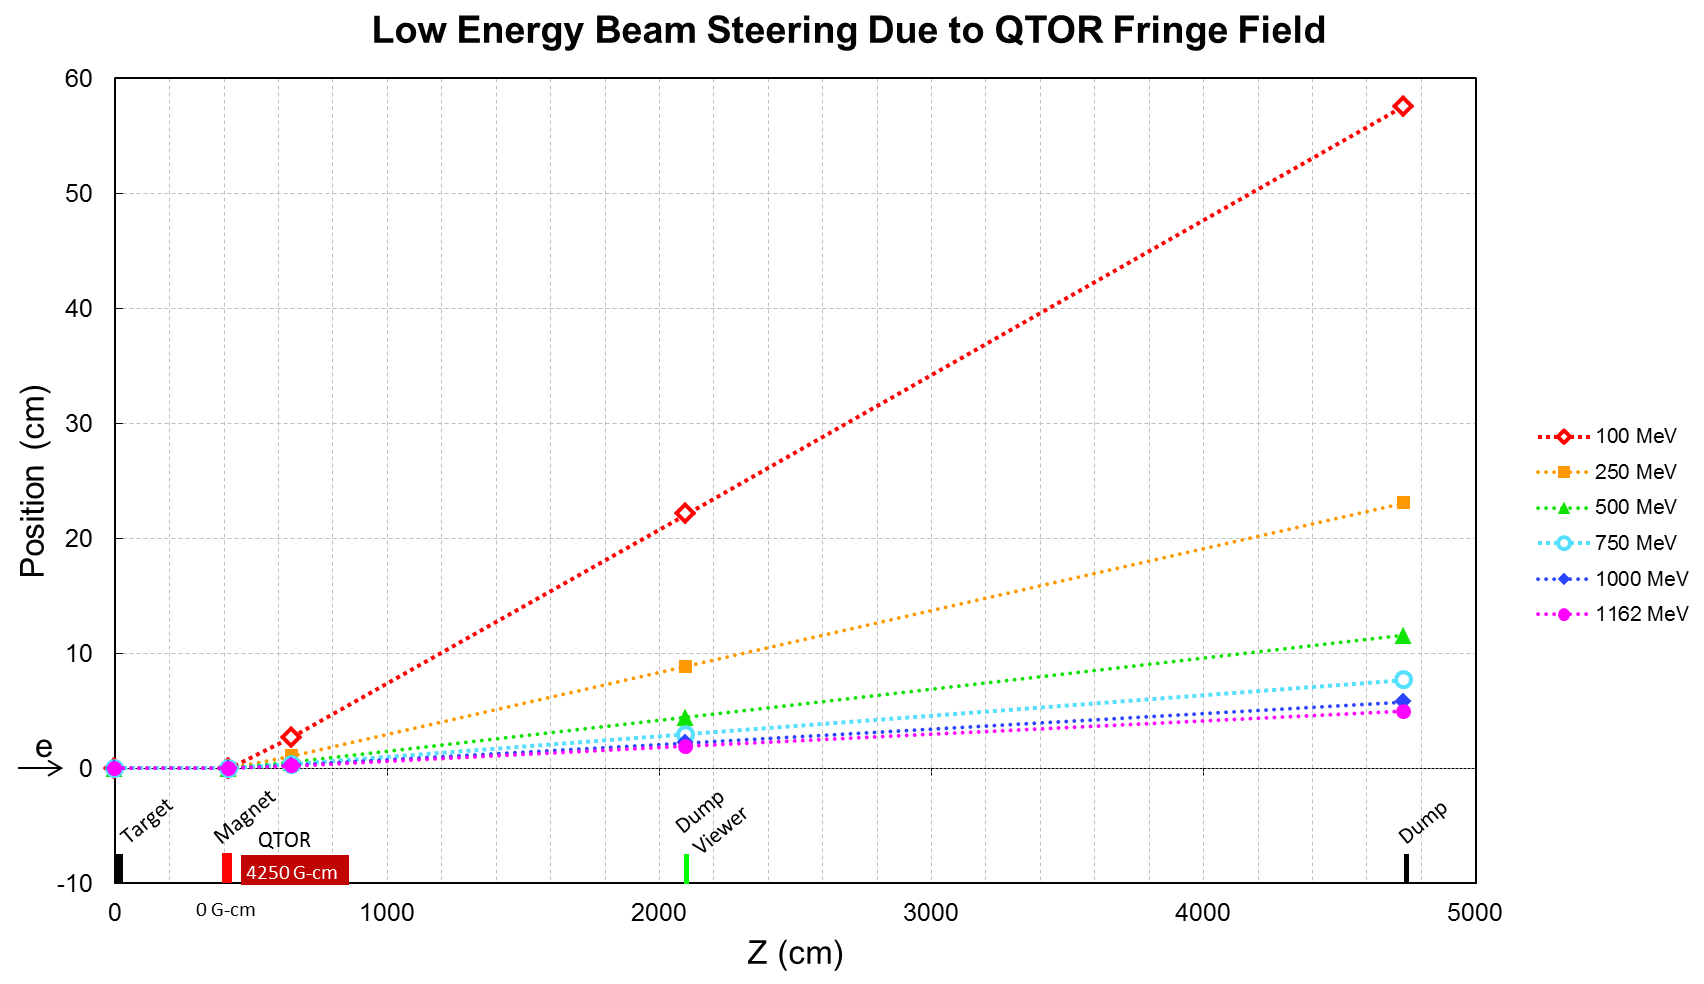
\includegraphics[trim=0.1cm 0.1cm 0.1cm 0.1cm, clip=true,width=14.5cm]{figures/qtor_allenergy_0Gcm}
		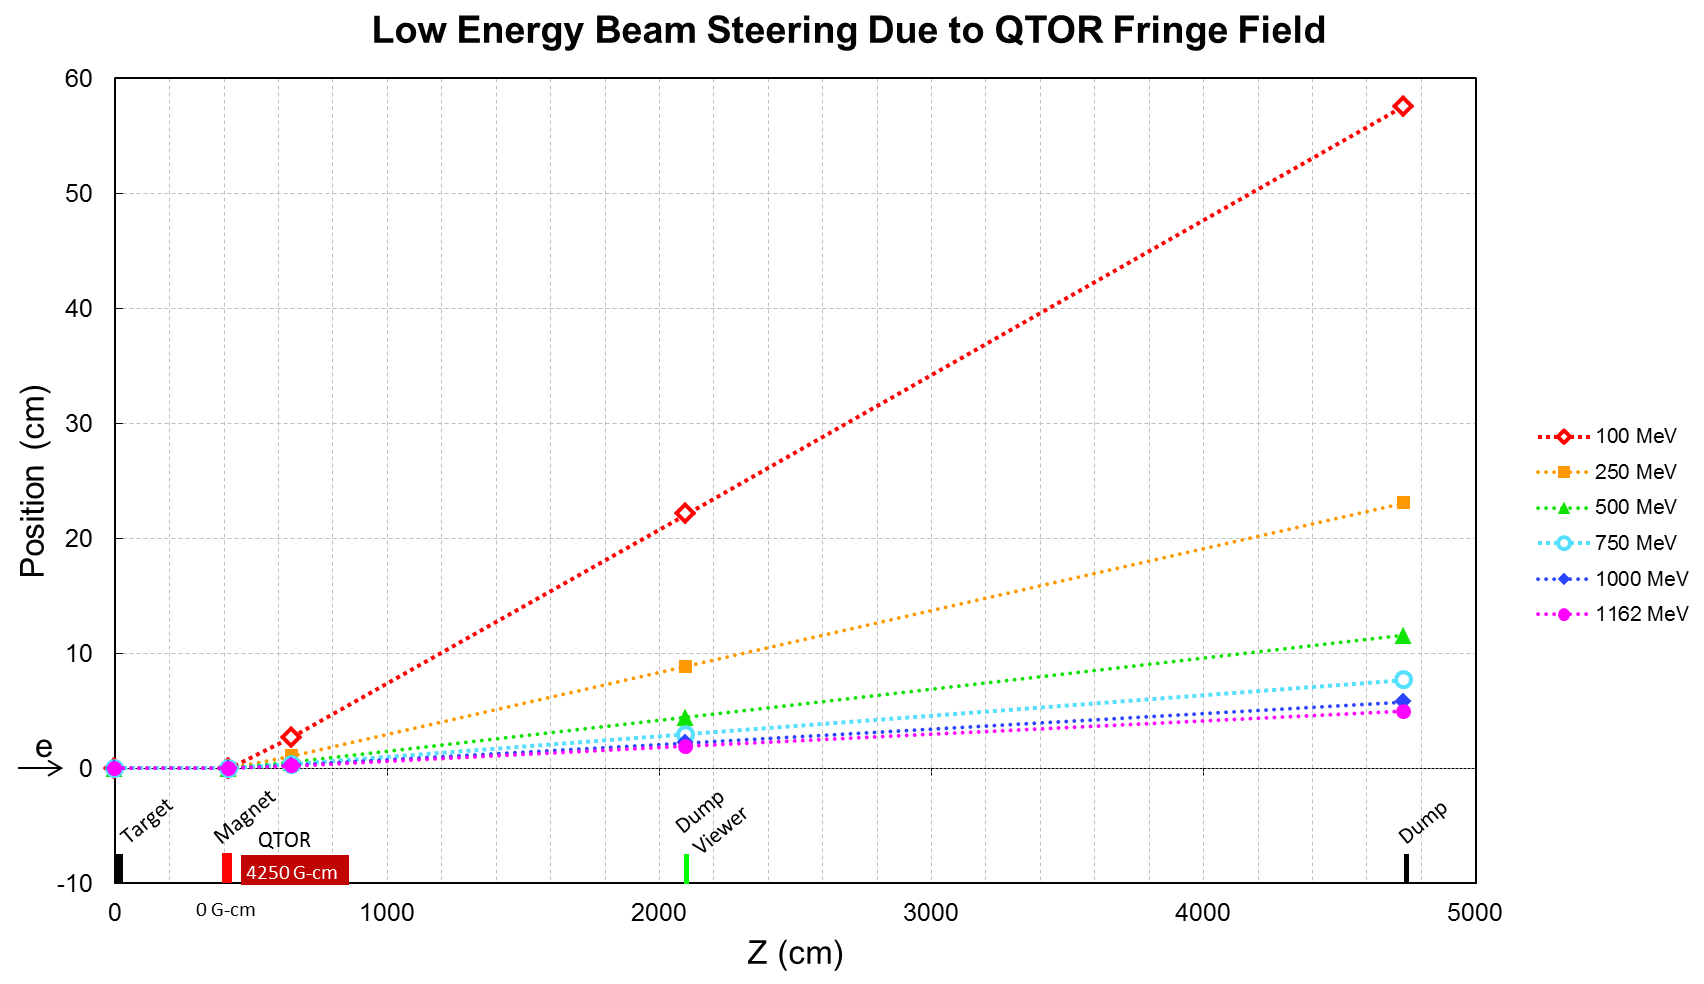
\includegraphics[width=15.0cm]{figures/qtor_allenergy_0Gcm}
	\end{center}
	\caption
%		[QTor all energy 0~G-cm.]
		{A simulation of the beam steering due to QTor fringe field (4250 Gauss-cm) for the primary electron beam (1.2 GeV) is shown in purple. The simulated tracks of the low energy electrons are also shown here. The primary beam spot moved $\sim$2~cm on the dump viewer between QTor OFF and ON.}
		\label{fig:qtor_allenergy_0Gcm}
\end{figure}
\end{singlespace}


%%%%%%%%%%%%%%%%%%%%%%%%%%%%%%%%%%%%%%%%%%%%%%%%%%%%%%%%%%%%%
\section{QTOR Fringe Field and Optics Change\index{QTOR!Fringe Field and Optics Change}}
\label{QTOR Fringe Field and Optics Change}

There was a vacuum leak activated by heating due to low energy electrons near the beam dump during Run 1.  This unplanned event forced a delay in the experiment for months. 
Smaller bellows diameter with two stainless steel flanges might have been activated due to low energy electrons coming from upstream which might have caused the vacuum leak. It was found that the QTor has a non-zero field integral along the beam axis and might have deflected the low energy electrons in the dump viewer flanges. So, the plan of the collaboration was to improve the hardware assembly near the beam dump with a larger bellows diameter (see Figure~\ref{fig:vacuumLeakProblem} top panel) before Run 2. The new structure was built to minimize the stainless exposure, and low energy electrons coming from radiative tail stripe landed on aluminum, which helped to reduce the activation (see Figure~\ref{fig:vacuumLeakProblem} bottom panel). Another strategy was to design and build a corrector magnet to counter steer the fringe filed of the QTor.

\begin{singlespace}
\begin{figure}[!h]
	\begin{center}
		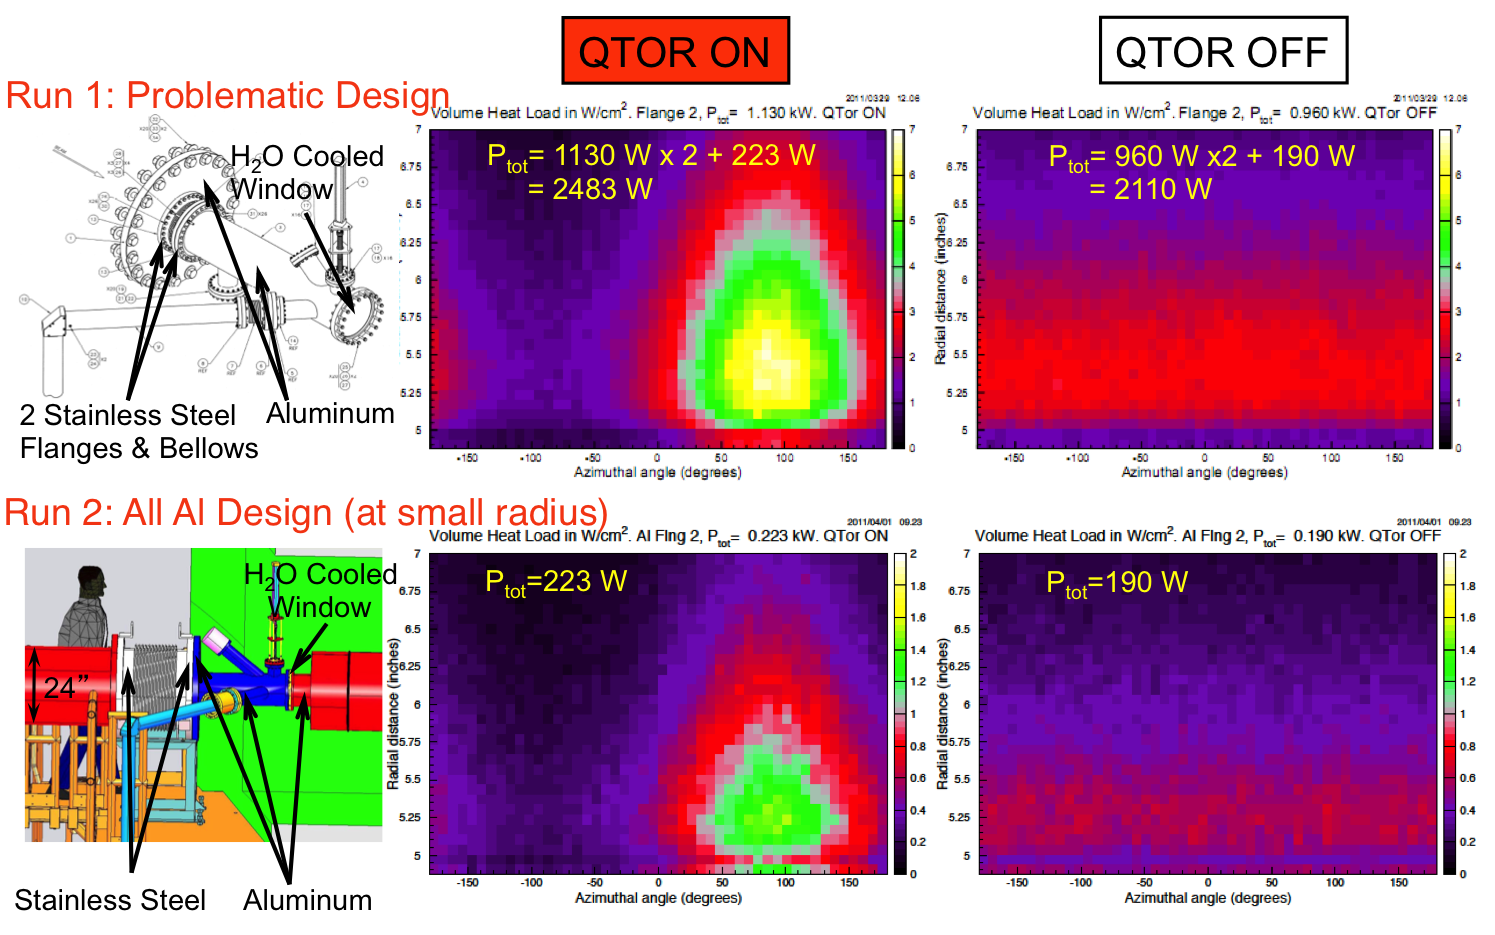
\includegraphics[width=15.0cm]{figures/vacuumLeakProblem}
	\end{center}
	\caption
%		[Bellows hardware and vacuum heat load before and after the activation.]
		{Bellows hardware and vacuum heat load before and after the activation. The top panel shows the Run 1 hardware of the bellows in the left and volume heat loads in the flange during QTor ON and OFF, respectively. Run2 bellows hardware and volume heat loads are shown in the bottom panel.}
		\label{fig:vacuumLeakProblem}
\end{figure}
\end{singlespace}

At the beginning of the experiment, it was observed that QTor steers the forward beam and one important question was to examine whether the steering could be caused by the expected QTor fringe field along the beam axis, or whether the steering indicates misalignment or motion of any coils. The primary beam (1.2~GeV) spot moved $\sim$2~cm on the dump viewer between QTor OFF and ON. The magnet steered the beam up and right towards the observed hot spot in the dump viewer (see Figure~\ref{fig:vacuumLeakProblem} top panel). The steering implies a residual field integral of 4250~Gauss-cm in QTor. The natural fringe field near the axis of an ideal eight-fold toroid scales like $r^{7}$~\cite{elog:rob_qtor2}, and was not strong enough to cause the observed steering unless the beam was many centimeters away from the axis for most of the length of the toroid. However, a radial shift of one coil by 3~mm generates a large enough residual field on the axis to steer the beam as observed. 
%The idea of this analysis is to estimate beam steering due to QTor fringe field assuming a field of 4500 Gauss-cm along the beam axis using OptiM.
The effect of the QTor fringe field (4250 Gauss-cm) along the beam axis was simulated using OptiM~\cite{elog:nur_qtor3}. The simulation conditions were as follows: 

\begin{itemize}
\doublespacing
\item QTor and dump viewer in the OptiM model were added to the Q-weak main input deck~\cite{jay_communication} for this analysis.
\item No microscopic model of the QTor field symmetry breaking was used. The QTor region was treated as a 4~m long dipole with a 4250 Gauss-cm field integral.
\item Earth's magnetic field was ignored in the simulation.
\end{itemize}

A beam steering of $\sim$2~cm at the beam dump viewer due to QTor fringe field (4250 Gauss-cm) was observed in the simulation for the primary electron beam (1.2~GeV) and confirmed the earlier observation. The effect of the fringe field on lower energy electrons was much higher, and the simulated tracks are shown in Figure~\ref{fig:qtor_allenergy_0Gcm}~\cite{elog:nur_qtor4}. 

\begin{singlespace}
\begin{figure}[!h]
	\begin{center}
		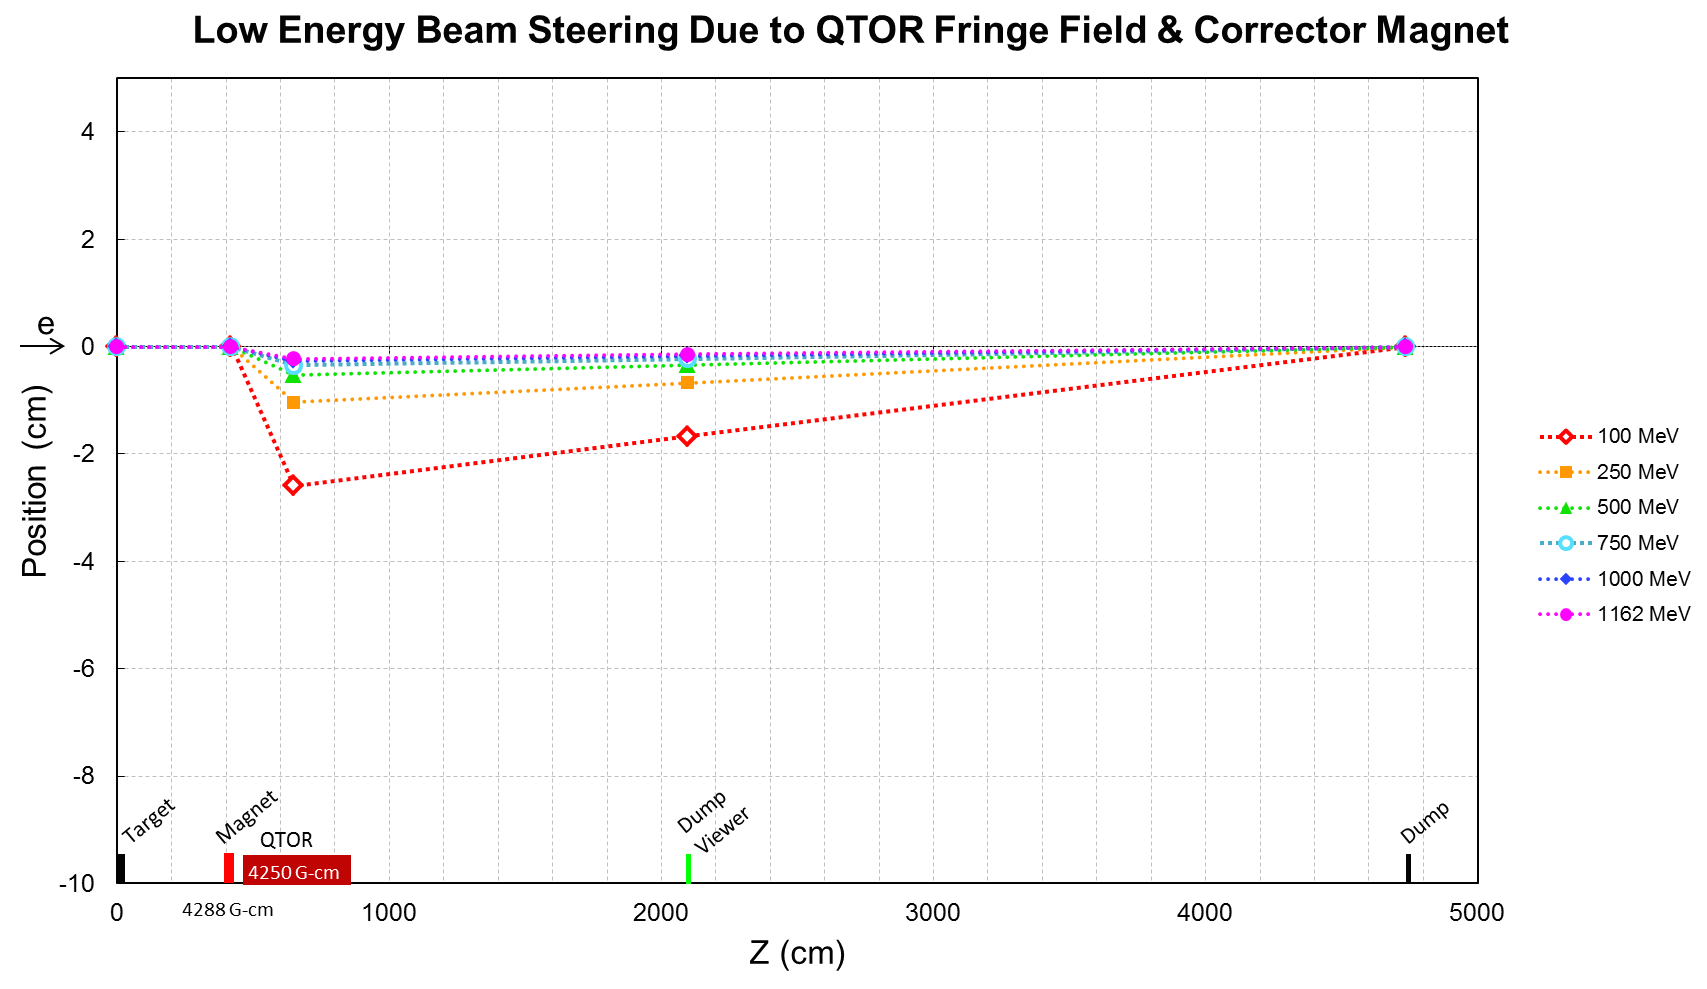
\includegraphics[width=15.0cm]{figures/qtor_allenergy_4000Gcm_sacle_dump}
	\end{center}
	\caption
%		[QTor all energy 4000Gcm dump.]
		{The simulated tracks of the primary and low energy electrons, after inserting a corrector magnet in front of the QTor with a magnetic field of 4000 Gauss-cm in the simulation, are also shown here. The corrector magnet focuses electron tracks on the dump by correcting the fringe field (4250 Gauss-cm) in QTor.}
		\label{fig:qtor_allenergy_4000Gcm_sacle_dump}
\end{figure}
\end{singlespace}

\subsection{QTOR Corrector Magnet\index{QTOR!Corrector Magnet}}
\label{QTOR Corrector Magnet}

%\subsubsection{TOSCA Design\index{TOSCA}}
%\label{TOSCA Design}

The next step was to design a corrector magnet that could suppress the fringe field in the QTor and fit into existing beamline structure. The ideal location for the corrector magnet was simulated to be in front of the QTor~\cite{elog:nur_qtor5}.
The estimated magnet field strength for the corrector magnet, placed before QTor, to compensate beam steering due to the QTor fringe field was $\sim$4000~Gauss-cm. The effect of the corrector magnet on the QTor fringe field is shown in Figure~\ref{fig:qtor_allenergy_4000Gcm_sacle_dump}.
%Estimation of the magnet field strength placed before QTor to compensate beam steering due to QTor fringe field assuming a field of 4250 Gauss-cm along the beam axis using OPTIM.
Besides containing the primary electrons, the corrector magnet also helped in suppressing the lower energy electrons~\cite{elog:nur_qtor6}. The corrector magnet had a bedstead structure and was designed using TOSCA~\cite{elog:nur_qtor7, elog:nur_qtor8} (see Figure~\ref{fig:qtor_corrector_vector}).

%\begin{itemize}
%\doublespacing
%\item Current through inner coil 2600~A, outer coil -1000~A.
%\item Inner coil length along Z = 8~cm, radius along X = 14~cm, radius along Y = 20~cm.
%\item Outer coil length along Z = 10~cm, radius along X = 28~cm, radius along Y = 32~cm.
%\item Inner coil cross section 2.5x4.0~cm$^{2}$, outer coil cross section 2.5x2.5~cm$^{2}$.
%\end{itemize}
%
%\begin{table}[!h]
%\begin{center}
%  	\caption
%  	[The design parameters for the QTor corrector magnet.]
%  	{The design parameters for the QTor corrector magnet.}
%  \begin{tabular}{ l | c | c | c | c | c }
%    \noalign{\hrule height 1pt}
%%    \multirow{2}{*}{Channels}  & False Asymmetry & \multirow{2}{*}{Sensitivity} & Nonlinearity & \multirow{2}{*}{Electronic Noise} \\
%    \multirow{2}{*}{Coils} &	Current	&	X-radius	&	Y-radius	&	Z-length	& Cross section	\\ 
%            &	[A]		&	[cm]		&	[cm]		&	[cm]		&	[cm$^{2}$]	\\ 
%    \noalign{\hrule height 1pt}
%    Inner 	&	2600		& 14.0		&	20.0		&	8.0		&	2.5$\times$4.0	\\
%    Outer 	&	-1000	& 28.0		&	32.0		&	10.0		&	2.5$\times$2.5	\\
%    \noalign{\hrule height 1pt}
%  	\end{tabular}
%  \label{tab:QTorCorrectorMagnetParameters}
%\end{center}
%\end{table}

\begin{table}[!h]
\begin{center}
  	\caption
%  	[The design parameters for the QTor corrector magnet.]
  	{The design parameters for the QTor corrector magnet.}
  \begin{tabular}{ l | c | c }
    \noalign{\hrule height 1pt}
    Parameters	&	Inner	& Outer	\\ 
    \noalign{\hrule height 1pt}
    X-radius [cm]	& 	14.0		&	28.0 \\
    Y-radius [cm]	& 	20.0		&	32.0 \\
    Z-length [cm]	& 	8.0		&	10.0 \\
    Cross section [cm$^{2}$]	& 	2.5$\times$4.0	&	2.5$\times$2.5 \\
    Current [A]	&	2600 &	-1000 \\ 
	No. of turns		& 	240		&	150	\\
	Length per turn [cm]	&	132.48	&	240.96 \\
	Current per turn	[A]	&	10.84	&	6.67 \\
	Resistance [$\Omega$]	&	1.15	&	1.30 \\
	Total length [cm]	&	34947	&	39727 \\
	Mass [kg]		&	11.87	&	13.49 \\
	Power [W]		&	149.56	&	64.38 \\
	Voltage drop [V]	&	13.79	&	9.65 \\
	Temperature rise [K/s]	&	3.23$\times$10$^{-2}$	&	1.22$\times$10$^{-2}$ \\
    \noalign{\hrule height 1pt}
  	\end{tabular}
  \label{tab:QTorCorrectorMagnetParameters}
\end{center}
\end{table}


The design parameters for the QTor corrector magnet are summarized in Table~\ref{tab:QTorCorrectorMagnetParameters}. There were some constraints designing the corrector magnet as follows:

\begin{itemize}
\doublespacing
\item The space available for the corrector magnet was 25.4~cm along Z-direction. %See attachment 8. Beam direction and sketch of a pair of coils is shown on the figure.
\item The lower edge of the collimator opening was $\sim$40 cm from the center of the beam pipe.
\item The beam pipe diameter inside QTor was 27.4~cm.
\item The corrector magnet had to be non-magnetic material to reduce EM interference. 
%\item 
\end{itemize}

\begin{figure}[!h]
	\begin{center}
		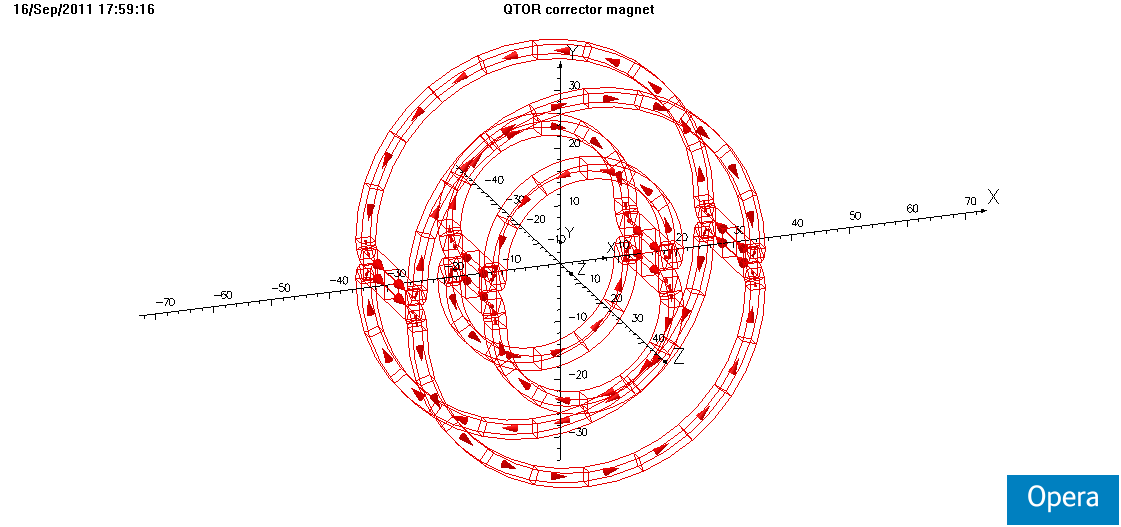
\includegraphics[width=15.0cm]{figures/qtor_corrector_vector}
	\end{center}
		\caption
%		[QTOR corrector magnet design.]
		{A 3-dimensional view of the QTOR corrector magnet design is shown here. The radius of the inner coil is half of the outer coil radius. The two coils carry currents in opposite direction (the direction of the current is shown by the arrows).}
		\label{fig:qtor_corrector_vector}
\end{figure}

The corrector magnet was designed to fit in the available space in front of the QTor and was capable of producing the desired field to counter steer the QTor fringe field. The power dissipation, voltage drop, temperature rise, and other important parameters associated to the coils were calculated and showed promising behavior (more details in~\cite{elog:nur_qtor9}). The corrector magnet sensitivity to position and angle changes in space was simulated using TOSCA by moving each coil individually in all possible orientations. The simulation yields the magnet to be mostly insensitive to the position and angle changes (more details in~\cite{elog:nur_qtor10}). 

The field integral produced by the corrector magnet is shown in Figure~\ref{fig:qtor_corrector_field_integral}. The Figure~\ref{fig:qtor_corrector_field_integral} also shows the field along X and Y direction at the collimator opening. The variation of magnetic field along the different octants has also been studied~\cite{elog:nur_qtor11} (see Figure~\ref{fig:qtor_corrector_field_integral_variation}, APPENDIX~\ref{QTOR}). The field seems to decay very fast along the radial direction. The summary of the magnet design can be found in~\cite{elog:nur_qtor12}. %As the hardware in the beam dump region was improved and due to schedule pressure, the corrector magnet was not finally built.
As the hardware in the beam dump region was improved, it was decided not to build the corrector magnet in order to adhere to the schedule.

%~\cite{elog:rob_qtor2, elog:nur_qtor3, elog:nur_qtor4, elog:nur_qtor5, elog:nur_qtor6, elog:nur_qtor7, elog:nur_qtor8, elog:nur_qtor9, elog:nur_qtor10, elog:nur_qtor11, elog:nur_qtor12}

%We have discovered recently that QTor steers the forward beam. In the attached note (which I could typeset if requested, but for now I'm posting handwritten), I examine whether that steering could be caused by the expected QTor fringe field along the beam axis, or whether the steering indicates misalignment or motion of any coils. The steering implies a field integral of 45 Gauss-meters. The natural fringe field near the axis of an ideal eight-fold toroid scales like r7, and isn't strong enough to cause the observed steering unless the beam is many centimeters from the axis for most of the length of the toroid. However a radial shift of one coil by 3 mm generates a large enough residual field on axis to steer the beam as observed. In other words, we should have seen this coming. - Rob

%Recently we discovered QTor steers the forward beam. We tried to examine whether this steering is due to expected QTor fringe field along the beam axis, or it indicates misalignment or motion of any QTOR coils. The steering implies a field integral of 4500 Gauss-cm. See more details in [1]. In this analysis we tried to predict the effect of QTor fringe field (4500 Gauss-cm) along the beam axis Using OptiM simulation.

%We have discovered recently that QTor steers the forward beam. In the attached note (which I could typeset if requested, but for now I'm posting handwritten), I examine whether that steering could be caused by the expected QTor fringe field along the beam axis, or whether the steering indicates misalignment or motion of any coils. The steering implies a field integral of 45 Gauss-meters. The natural fringe field near the axis of an ideal eight-fold toroid scales like r7, and isn't strong enough to cause the observed steering unless the beam is many centimeters from the axis for most of the length of the toroid. However a radial shift of one coil by 3 mm generates a large enough residual field on axis to steer the beam as observed. In other words, we should have seen this coming. - Rob ELOG QTor 2

\begin{figure}[!h]
	\begin{center}
		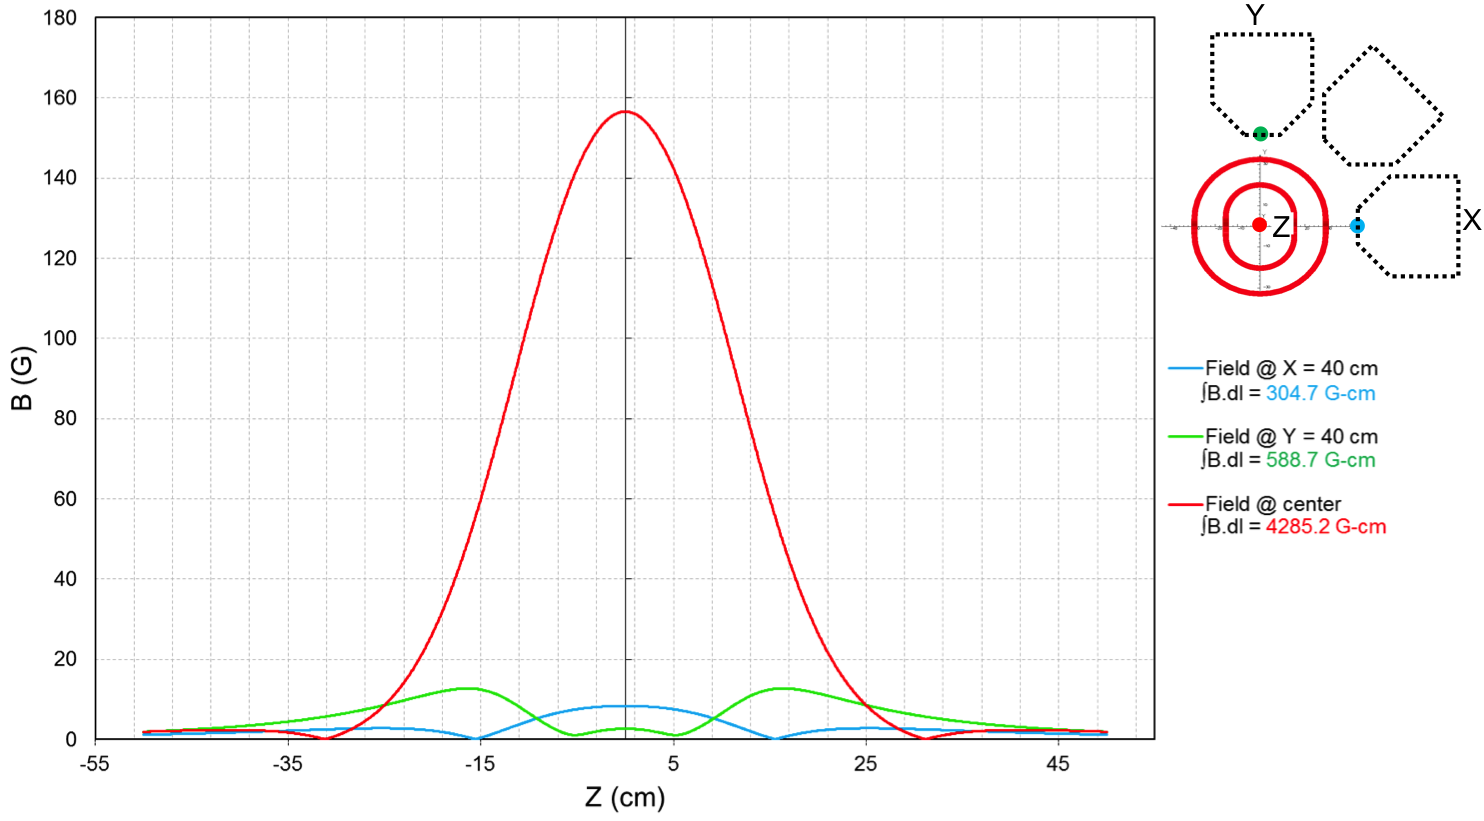
\includegraphics[width=15.0cm]{figures/qtor_corrector_field_integral}
		\caption
%		[QTor corrector field integral.]
		{The field integral of the QTOR corrector magnet along the X, Y, and Z axes are shown in blue, green, and red, respectively. The filed along the Z axis was measured along the center of the magnet, whereas the filed along X and Y axes were measured at collimator openings (40 cm away from the center).}
		\label{fig:qtor_corrector_field_integral}
	\end{center}
\end{figure}

%\begin{singlespace}
%\begin{figure}[!thp]
%	\begin{center}
%		\subfigure{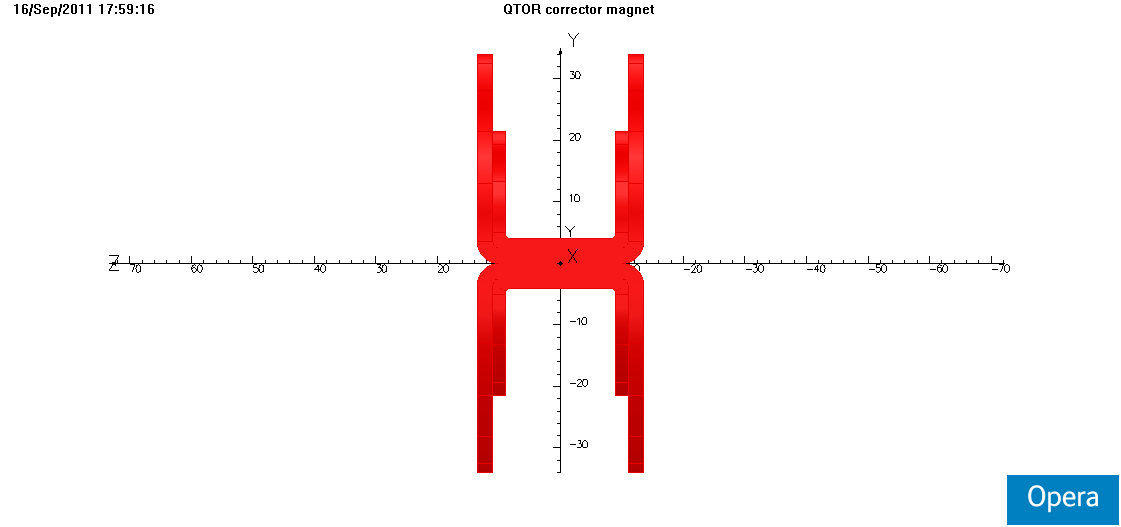
\includegraphics[width=7.0cm,height=3.4cm]{figures/qtor_corrector_model_yz}}
%		\quad
%		\subfigure{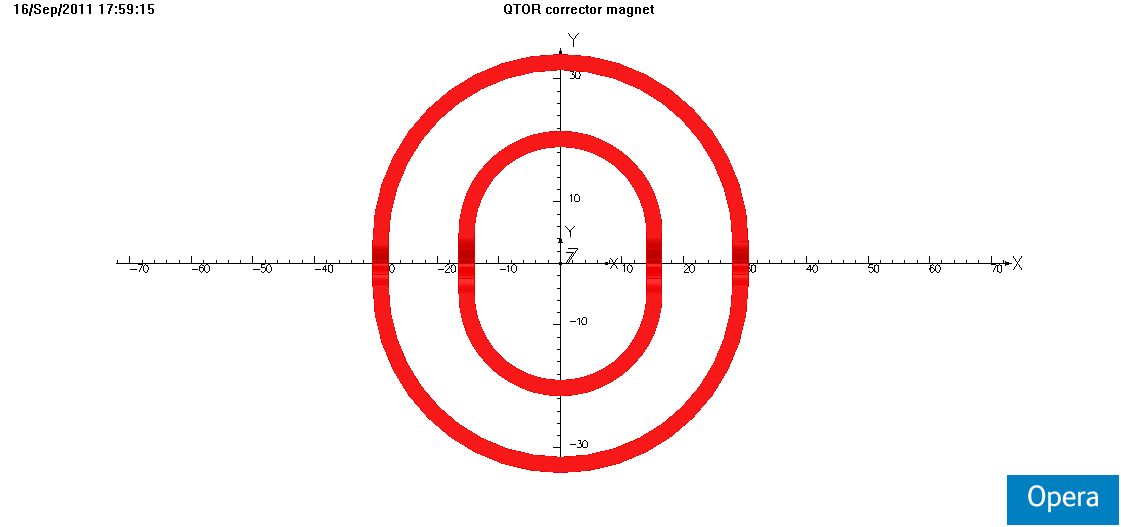
\includegraphics[width=7.0cm,height=3.4cm]{figures/qtor_corrector_model_xy}}
%		\caption{Magnet design}
%		\label{fig:qtor_corrector_design}
%	\end{center}
%\end{figure}
%\end{singlespace}

%We have already seen QTor steers the forward beam due to fringe field [1, 2]. We have predicted the effect of QTor fringe field (4250 Gauss-cm) along the beam axis using OptiM simulation [2] and supported Rob's pencil model. In this analysis we want to approach further and want to investigate the different effects of this fringe field on low energy electrons.

%Analysis conditions were as follows: 
%
%\begin{itemize}
%\doublespacing
%\item QTor and dump viewer in the OptiM model has been added for this analysis
%\item No microscopic model of the QTor field symmetry breaking was used. We treated the QTor region as a 4m long dipole with Rob's suggested field integral, confirming his estimate.
%\item Earth's magnetic field has not been considered in the model.
%\end{itemize}

%* QTor and dump viewer in the OptiM model has been added for this analysis. See details in [2].
%
%* No microscopic model of the QTor field symmetry breaking was used. We treated the QTor region as a 4m long dipole with Rob's suggested field integral, confirming his estimate.
%
%* Earth's magnetic field has not been considered in the model.

%Low energy electron scattering due to 4250 G-cm field at QTor magnet. The points are fitted with
%polynomial 2. The horizontal axis is shows the different beamline element. The Q-weak target is at zero and beam is coming from left. Different energies are shown in different colors (Colors are chosen according to energy. Convention is Violet – 1162 [nominal], Indigo – 1000, Blue – 750, Green – 500, Orange – 250 and Red – 100 MeV). As expected low energy electrons are deflected much more than high energy electrons. 
%
%Motivation: We have already seen QTor steers the forward beam due to fringe field [1, 2]. We have predicted the effect of QTOR fringe field (4250 Gauss-cm) along the beam axis using OPTIM simulation [2,3]. In this analysis we want to add a corrector magnet in front of QTOR and investigate the effects of this magnet on fringe field on electrons.
%
%Figure 1: Beam trajectory after applying ZERO filed in the corrector magnet in front of QTor. 
%
%Figure 2: Beam trajectory after applying a filed of 4000 G-cm in the corrector magnet in front of QTor. Its mainly focusing the trajectories at the dump viewer. 
%
%Figure 3: Beam trajectory after applying a filed of 4000 G-cm in the corrector magnet in front of QTor to focus at the dump viewer. Same as Figure 2, just a zoomed in version for better visualization.
%
%Figure 4: Beam trajectory after applying a filed of 4288 G-cm in the corrector magnet in front of QTor. Its mainly focusing the trajectories at the dump window. 
%
%Figure 5: Beam trajectory after applying a filed of 4288 G-cm in the corrector magnet in front of QTor to focus at the dump window. Same as Figure 4, just a zoomed in version for better visualization.

%We have investigated the effects of a magnet in front of QTor on different energy electrons [4]. In
%this analysis we want to vary the  magnetic field of corrector magnet in front of QTor and investigate the
%effects of this field variation on electrons.
%
%Figure 1: Beam trajectory due to different fields in the corrector magnet for a single energy electrons. Then the plot is animated over different beam energies. The beam energy is written on the headings of the plots and different magnetic fields are shown in different colors and symbols are shown in the legend section (right hand side) of the plots. 
%
%At the end we may not approach for a magnet in front of QTor due to its far field effect. Later we may search for a different place (most likely downstream, as we don't have enough space upstream of QTor) rather than just before QTOR.
%
%
%
%Motivation: We found QTOR steers the forward beam most probably due to misalignment of QTor coils [1]. We have already investigated the effects of a magnet in front of QTOR for primary beam as well as for different energy Moller electrons [2, 3, 4 and 5]. Here we tried to design a magnet we discussed in [4] and [5].
%
%Figure 1: 3D view of QTOR corrector magnet. The current directions for the coils are shown by the arrows. 
%
%Figure 2: QTOR corrector magnet along YZ plane. Length along Z-direction (available space for magnet is 25.4 cm) is shown in this figure.
%
%Figure 3: QTOR corrector magnet along XY plane. Magnetic field perpendicular to Z- plane is also shown in a polar patch of radii 40 – 90 cm.
%
%Figure 4: QTOR corrector magnet field integral along a line in Z- direction (from -50 to +50 cm) at X = 40 cm and Y = 0 cm.
%
%Figure 5: QTOR corrector magnet field integral along a line in Z- direction (from -50 to +50 cm) at X = 0 cm and Y = 40 cm.
%
%Figure 6: QTOR corrector magnet field integral along a line in Z- direction (from -50 to +50 cm) at X = 28.3 cm and Y = 28.3 cm (diagonal).
%
%Figure 7: QTOR corrector magnet field integral along a line in Z- axis (from -50 to +50 cm).
%
%Figure 8: Possible QTOR corrector magnet location. The arrow represents beam direction.
%
%Motivation: We discussed our corrector magnet design in [1]. Here we tried to calculate the power dissipation, voltage drop and temperature rise and other important parameters of the coils. 
%
%Motivation: We showed our corrector magnet design in [1]. Here we tried to get an estimate of corrector magnet sensitivity to position or angle using TOSCA. 
%
%
%Motivation: Corrector magnet design has been shown in [1]. We tried to see the profile of magnetic field along the line of collimator opening using TOSCA. ~\ref{OPTIM}




%%%%%%%%%%%%%%%%%%%%%%%%%%%%%%%%%%%%%%%%%%%%%%%%%%%%%%%%%%%%%
\section{BPM Resolution}
\label{BPM Resolution}

The BPMs in front of the target e.g; 3H09B, 3H09, 3H07C, 3H07B, and 3H07A were used for the linear regression as well as for the calculation of the virtual target BPM.  Hence, it was important to know their position and angle resolutions. The BPM position resolution was extracted from the collected production data and the angle resolution was simulated using the relation between the position and the angle resolution at a fixed beam current.

\subsection{Position Resolution\index{BPM!Position Resolution}}
\label{Position Resolution}
The target BPM is a virtual BPM calculated using five BPMs in the drift region (more details on virtual target BPM in section~\ref{Beam Position Monitor} and \cite{buddhini_qweak}). The position resolution of the BPM in front of the target was extracted by observing the residual of beam position differences (between two helicity states) on any BPM and the orbit projected from the target. This is expressed in Equation~\ref{equ:bpmPositionResolution} (see cartoon diagram in Figure~\ref{fig:bpmPositionResolutionCartoon}). 

\begin{equation} \label{equ:bpmPositionResolution}
\begin{split}
\text{BPM resolution} \approx \sigma_{Residual} = diff_{BPM} - \text{Orbit Position Differences} \\
\text{Orbit Position Differences} = (Z_{BPM} - Z_{Tgt}) diff_{TgtSlope} + diff_{Tgt}
\end{split}
\end{equation}

%\begin{equation} \label{equ:bpmPositionResolution2}
%\text{Orbit Position Differences} = (Z_{BPM} - Z_{Tgt}) diff_{TgtSlope} + diff_{Tgt}
%\end{equation}


\begin{singlespace}
\begin{figure}[!h]
	\begin{center}
	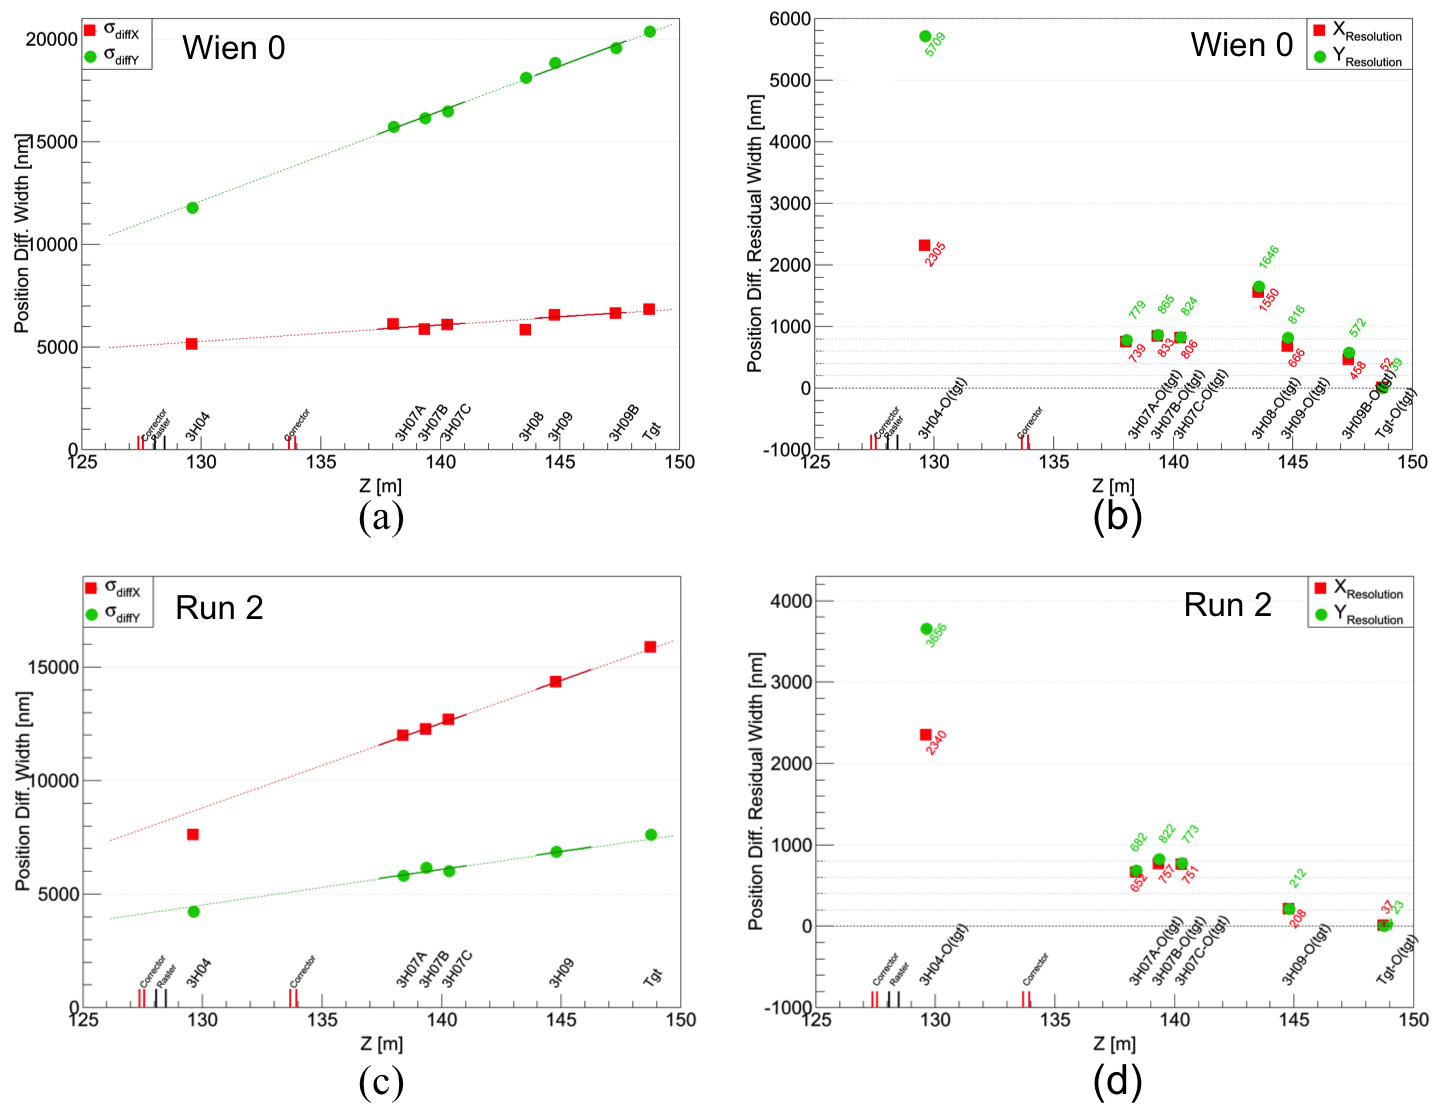
\includegraphics[width=15.0cm]{figures/bpmPositionResolution}
	\end{center}
	\caption
%	[BPM position resolution.]
	{BPM position resolution. (a) Beam position differences for a typical one hour production run during Wien 0 at beam current of 145~$\mu$A. Error weighted pol1 fits are shown by solid lines. BPM 3H04, 08 and, Tgt are not included in the fit. Fit is extrapolated using dashed line to guide the view. (b) Extracted BPM resolutions using (a) are shown for Wien 0 at beam current of 145~$\mu$A. (c) and (d) show beam position differences and BPM resolution, respectively for Run 2 at beam current of 180~$\mu$A.}
	\label{fig:bpmPositionResolution}
\end{figure}
\end{singlespace}

\begin{singlespace}
\begin{figure}[!h]
	\begin{center}
	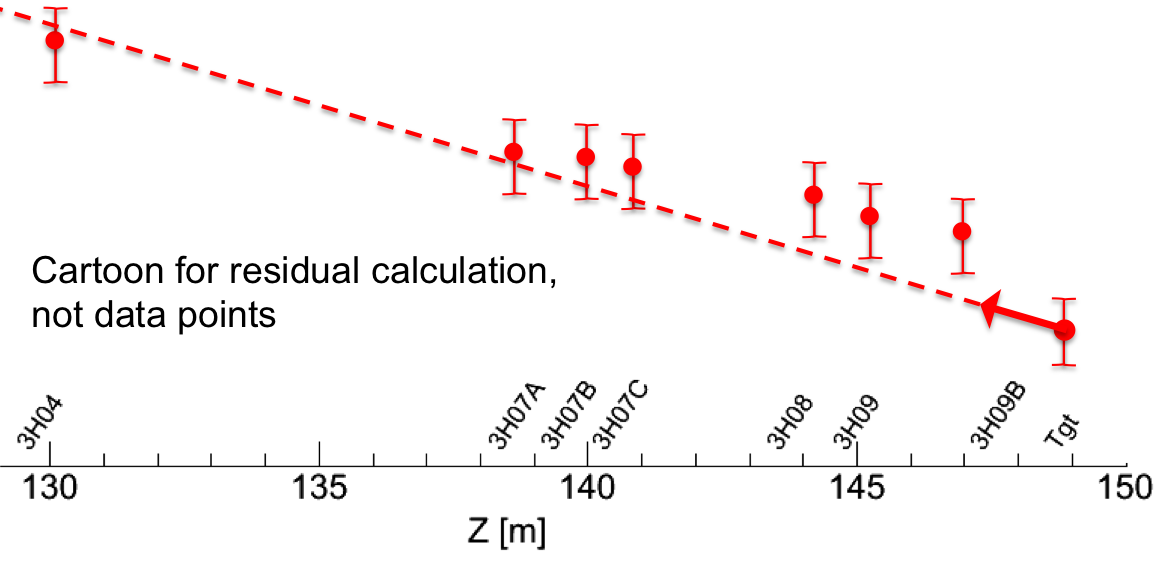
\includegraphics[width=10.0cm]{figures/bpmPositionResolutionCartoon}
	\end{center}
	\caption
%	[BPM resolution cartoon.]
	{BPM resolution cartoon.}
	\label{fig:bpmPositionResolutionCartoon}
\end{figure}
\end{singlespace}

Here $diff_{BPM}$ represents the beam position differences between two helicity states, $diff_{Tgt}$ represents the target position differences, $diff_{TgtSlope}$ represents the target slope differences, $Z_{BPM}$ is the location of the BPM in the beamline, and $Z_{Tgt}$ is the location of the target.

%* Y Resolution for 3H04 is poor and unstable. If this is real (D. Mack has doubts) it could be due to noise injected by corrector magnets.
The average BPM resolution using selective data samples from the commissioning phase of the experiment (Wien 0) is found to be 0.70	and 0.77 $\mu$m for X and Y, respectively at a fixed beam current of 145 $\mu$A. 
The position resolutions for all the BPMs in front of the target were stable during Wien 0 at fixed current and are summarized in Table~\ref{tab:positionResolution}. Y resolutions were quite similar to the X resolutions. 
%The resolution for the BPMs in front of the target are summarized in Table~\ref{tab:positionResolution}. 
An independent study of BPM 3H07B resolution by B. Waidyawansa~\cite{buddhini_resolution} has shown that the resolutions of 0.945~$\pm$~0.003, and 1.060~$\pm$~0.003 for X and Y, respectively at beam current 150 $\mu$A and roughly agrees with this result.
The BPM 3H09B had relatively good resolution but was not available during Run 2. The resolution for BPM 3H04 was poor, as shown in Figure~\ref{fig:bpmPositionResolution} (b). This inconsistency might be due to the noise injected by the existing corrector magnets between the BPM 3H04 and 3H07A. 
The BPM 3H08 had a different hardware compared to the other BPMs. Hence, the BPM 3H04 and 3H08 were not included for the construction of the virtual target BPM. 
The same analysis was repeated for Run 2 with a beam current of 180~$\mu$A, as shown in Figure~\ref{fig:bpmPositionResolution} (c) and (d). The BPM resolution improves with the increase in beam current. A study of the BPM resolution variation with beam current can be found in~\cite{buddhini_resolution}.

\begin{table}[!h]
\begin{center}
  	\caption
%	[BPM position resolution at beam current of 145~$\mu$A.]
  	{BPM position resolution at beam current of 145~$\mu$A.}
  \begin{tabular}{ l | c | c }
%    \hline
    \noalign{\hrule height 1pt}
    \multirow{2}{*}{BPM}  & X Resolution & Y Resolution \\
            & [$\mu$m]   & [$\mu$m] \\ 
%    \hline
    \noalign{\hrule height 1pt}
	3H09B		&	0.46		&	0.57 \\
	3H09			&	0.67		&	0.81 \\	
	3H07C		&	0.81		&	0.83 \\
	3H07B		&	0.83		&	0.87 \\
	3H07A		&	0.74		&	0.78 \\
	3H04			&	1.70		&	3.55 \\
%    \hline
    \noalign{\hrule height 1pt}
	Average (3H04 excluded)	&	0.70		&	0.77 \\
    \noalign{\hrule height 1pt}
  	\end{tabular}
  \label{tab:positionResolution}
\end{center}
\end{table}


\begin{singlespace}
\begin{figure}[!h]
	\begin{center}
	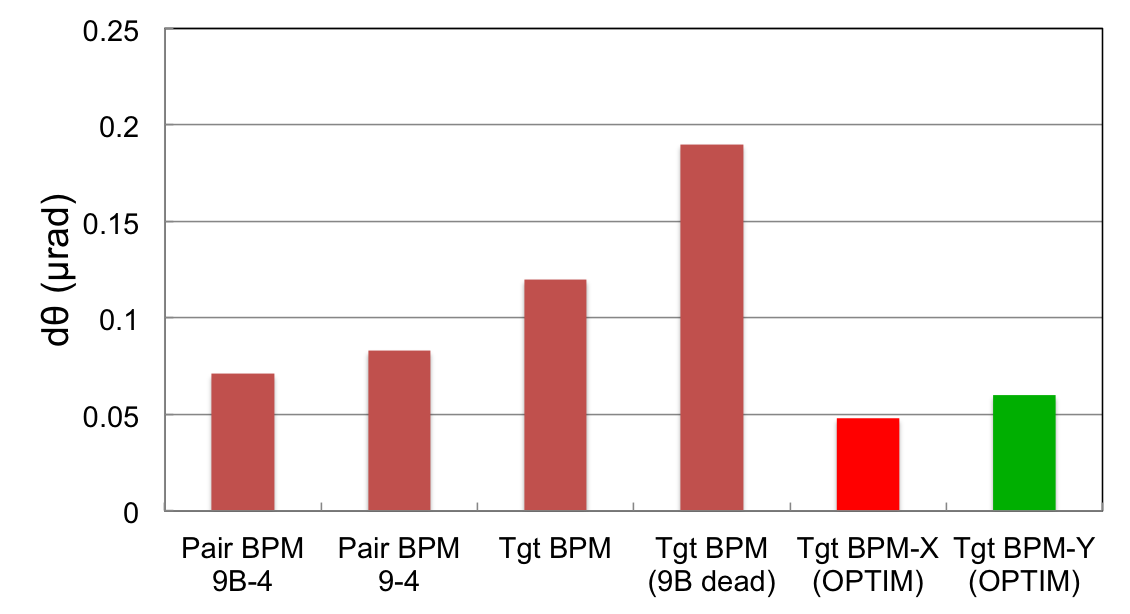
\includegraphics[width=15.0cm]{figures/bpmAngleResolution}
	\end{center}
	\caption
%	[Target BPM angle resolution at beam current of 180~$\mu$A.]
	{Target BPM angle resolution at beam current of 180~$\mu$A.}
	\label{fig:bpmAngleResolution}
\end{figure}
\end{singlespace}


\subsection{Target BPM Angle Resolution\index{BPM!Target BPM Angle Resolution}}
\label{Target BPM Angle Resolution}

The target BPM angle resolution was simulated using OptiM~\cite{OPTIM}. 
%The objective of this simulation is to estimate target BPM angle resolution.
In order to estimate the target BPM angle resolution, a relatively pure position measurement which corresponds to a pure angle measurement at the target was needed. 
%One such possible position measurement was found to be around the Compton region and chosen to be at BPM 3P02A from the simulation. 
A study of the strength sharing between angle and position in the various BPMs along the beamline for Wien 0 shows that the Compton BPMs (3P02A and B) were insensitive to the position at the target~\cite{presentation:nur_BPMAngleResolution_1779}. Then the known BPM position resolution and the transport matrices between the Compton BPMs and the target BPMs were used to estimate effective angle resolution. 
%* Need to find a relatively pure position measurement which corresponds to pure angle measurement at target.
%* With known BPM position resolution, effective angle resolution can be estimated.
% This estimate of target angle resolution using 3P02A is better than the angle resolution we have now.
Assuming the X(Y) position resolution to be 0.90 (0.96)~$\mu$m, the estimated target BPM X (Y) angle resolution at a fixed beam current of 180~$\mu$A is 0.048 (0.060)~$\mu$rad.
%
%\begin{equation} \label{equ:bpmXAngleResolution}
%\text{X-angle resolution} = 0.048~\mu\text{rad}
%\end{equation}
%
%\begin{equation} \label{equ:bpmXAngleResolution2}
%\text{Y-angle resolution} = 0.060~\mu\text{rad}
%\end{equation}
%
A simple model calculation, where the angle jitter at the target corresponds to a pure position at BPM 3P02A (without using the transport matrix), agrees with this simulation. 
%With the simple model where angle jitter at the target corresponds to pure position at 3P02A (without using transport matrix) also gives similar answer. 
%Target angle resolution using 3P02A is better than the angle resolution seen from regression. This simulation suggest incorporating BPM 3P02A into a regression scheme might be a good idea. 
The simulated target BPM resolution in this analysis is better than the existing calculation with other BPMs~\cite{presentation:mack_Wien0MDSensitivities_1776}. A comparison of the resolution using different BPM pairs is shown in Figure~\ref{fig:bpmAngleResolution}.

%Note: A study of strength sharing between angle and position in the various BPM's along the beamline (similar to Don’s study at ELOG 856) for wien0 (two runs from each slug) seems to show Compton BPMs (3P02A \& B) were insensitive to position on target.
%
%* OPTIM confirms that the Compton region should have appropriate optics for UVA’s angle-sensitive BPM (i.e. angle jitter at the target is transformed to position jitter at the BPM).
%
%* With X (Y) BPM position resolution of 0.90 (0.96)~$\mu$m, the effective target angle resolution is estimated to be 0.048 (0.060)~$\mu$rad. This is better than the angle resolution we have now, so we encourage UVA’s strategy of incorporating this BPM into a regression scheme.

%%%%%%%%%%%%%%%%%%%%%%%%%%%%%%%%%%%%%%%%%%%%%%%%%%%%%%%%%%%%%
\subsection{Consistency Check of the Target Variable\index{BPM!Target BPM Consistency Check}}
\label{Consistency Check of the Target Variable }

The most commonly used independent variables for the linear regression were target positions and angles. So it was important to check the consistency of the target variable since it was created using 5 BPMs in the drift region in the beamline over a span of 10~m upstream of the target (more details about target variable can be found in section~\ref{Beam Position Monitor} and in~\cite{nur_linear_reg, buddhini_qweak}). 
In order to check the consistency of the variable, the BPM differences used for the calculation were projected back to the target. A schematic diagram is shown in Figure~\ref{fig:bpmPositionResolutionCartoon}. The beam position differences and the BPM residuals from the projected orbit are shown in the Figure~\ref{fig:targetBPMConsistencyCheck}. The target BPM was consistent, but the target intercept in the Q-weak database sometimes was significantly inconsistent and made $\chi^{2}$/DOF of the fit worse. As in the regression or any of the Q-weak calculations, the intercept was not used, hence this inconsistency in the intercept did not make any impact on the physics result. A linear fit of the BPMs in front goes through the target BPM within 0.03~nm. The X position differences uncertainties are usually underestimated; this is necessary to assign the uncertainties in the regression. The BPM 3H04 effectively has the wrong units in the analysis software and a scale factor of 0.75 can eliminate this inconsistency. It is not very clear yet how big a problem this is for regression, since 3H04 was used in few regression schemes. The beam jitter was stable and Y jitter was larger than X jitter during Wien 0, but X jitter became larger than Y during Run 2. 
%The BPM 3H09B had very good resolution and was only available during Run 1 due to hardware failure. The resolution for the BPM 3H04 and 8 were high and had different hardware compare to other BPMs. BPM 3H07B resolution was $\sim$0.9~$\mu$m and agrees with an independent study~\cite{buddhini_resolution}. The corrector magnet between 3H04 and 3H07A seems to affect the resolution calculation. Resolution of other BPMs in front of target (in the drift region) seems reasonable.

\begin{singlespace}
\begin{figure}[!h]
	\begin{center}
	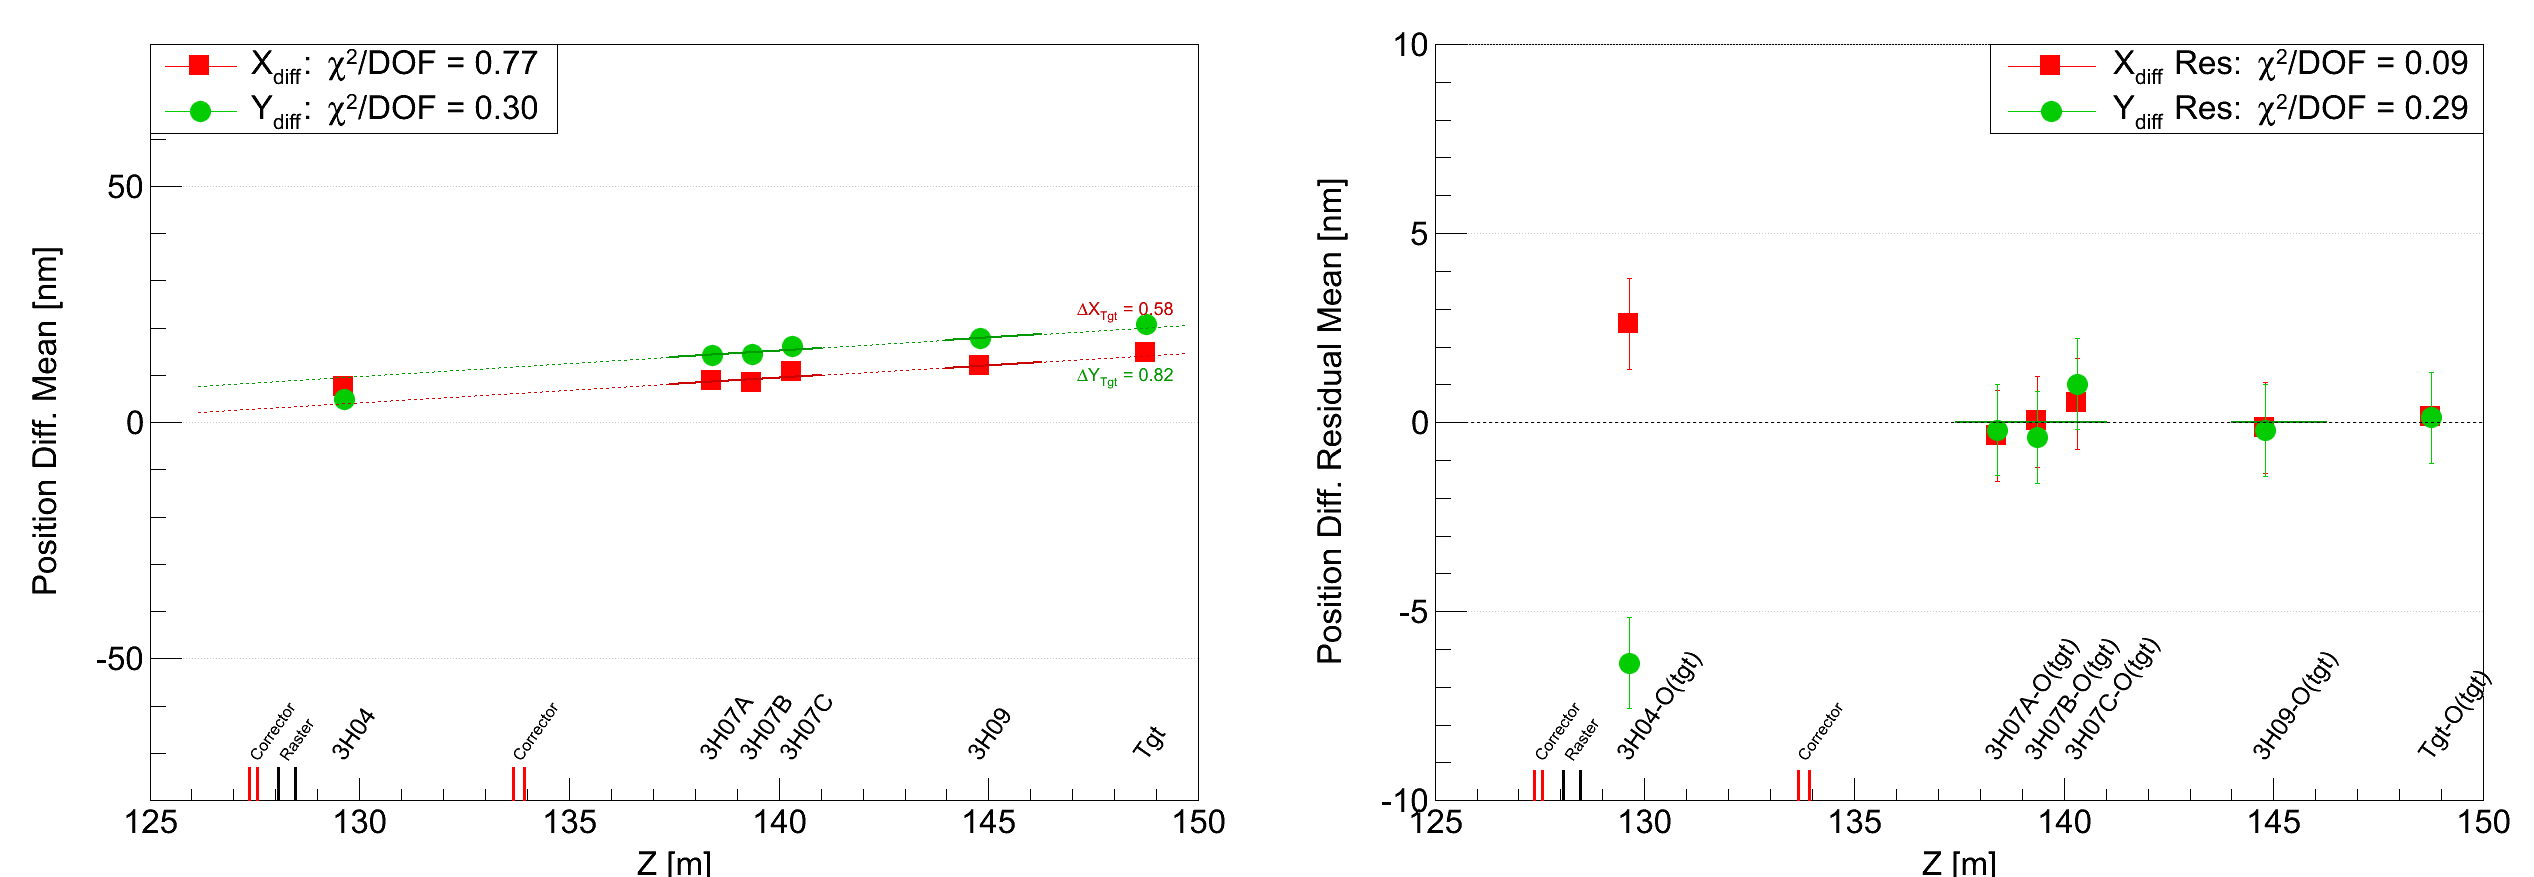
\includegraphics[width=15.0cm]{figures/targetBPMConsistencyCheck}
	\end{center}
	\caption
%	[Target BPM consistency check.]
	{Target BPM consistency check. Beam position differences for a typical one hour production run during Run 2 at beam current of 180~$\mu$A are shown in (a). Error weighted pol1 fits are shown by solid lines. BPM 3H04, 3H08 and, Tgt are not in the fit. Fit is extrapolated using dashed line to guide the view. The residual of the BPM position differences and extrapolated orbit from target are shown in (b).}
	\label{fig:targetBPMConsistencyCheck}
\end{figure}
\end{singlespace}

%Mack is investigating regression scheme dependence.
%Different regression schemes use different combinations of BPMs.
%Motivation was to check the consistency of the BPMs.
%* Can we reproduce the target BPM using BPMs in front?
%* Are the errors in helicity correlated differences estimated correctly?
%* What about BPM 3H04 which is used in several regression schemes?
%
%Target BPM itself is fine, it appears that intercept in DB sometimes significantly wrong and made these $\chi^{2}$/DOF worse. With new approach, without explicitly using intercept, $\chi^{2}$/DOF has improved.
%
%* Can we reproduce the target BPM using BPMs in front?
%Yes. A linear fit of the BPMs in front goes through target BPM within 0.03~nm.
%
%* Are the errors in helicity correlated differences estimated correctly?
%No. Xdiff errors are usually under estimated and we need to know it for assigning errors in regression.
%
%* What about BPM 3H04 which is used in several regression schemes?
%BPM 3H04 effectively has the wrong units. A scale factor of 0.75 fixes it. It is not clear yet how big a problem this is for regression.
%
%* How about beam jitter?
%Beam jitter was stable during slug 34 – 40. Some what different for slug 32, 33. Y jitter is larger than X jitter.
%
%To Do
%* Independently calculate BPM resolution (using rootfiles).
%
%* BPM 3H09B has good resolution. We will miss it during run2.
%* Resolution for 3H04 and 8 (different kind of BPM compare to others) are high.
%* For comparison resolution of BPM 3H07B from Buddhini (DocDB 1772) $\sim$0.9~$\mu$m matches
%with this calculation.
%
%3H04 Resolution:
%Current hypothesis: The corrector magnet between 3H04 and 3H07A might be affecting our calculation.
%
%BPM 3H04 and 3H02 jitter improved by gain adjustment but didn't improve resolution.
%
%* Using current method BPM 3H02 and 3H04 has poor resolution during wien0.
%* The corrector magnet between 3H04 and 3H07A seems to affect our resolution calculation. Resolution of other BPMs in front of target (in the drift region) seems reasonable.
%* An independent check will be helpful.



%%%%%%%%%%%%%%%%%%%%%%%%%%%%%%%%%%%%%%%%%%%%%%%%%%%%%%%%%%%%%
\section{Helicity Correlated Pedestal Analysis\index{Helicity!Helicity Correlated Pedestal}}
\label{Helicity Correlated Pedestal Analysis}

The Q-weak collaboration proposed to measure the small parity violating asymmetry ($\sim$250~ppb) in elastic electron-proton scattering precisely~\cite{qweak_proposal_2007}. The goal of the collaboration is to reduce any false asymmetry from various sources. One such potential source is helicity correlated pedestal differences for different detectors. The beam off detector yields at nominal operation and settings are known as pedestals of that detector. Pedestal can be determined by the preamplifier offset and backgrounds with beam off data. 
%The objective of the Q-weak experiment is to measure the parity violating asymmetry ($\sim$230~ppb) in elastic e+p scattering to determine the weak charge of proton with a $\sim$4\% combined statistical and systematic uncertainty ~\cite{qweak_proposal_2007}. The asymmetry predicted in Standard Model is very small and the Q-weak collaboration~\cite{website:qweak} has proposed to measure this asymmetry very precisely. The goal of the collaboration is to reduce any false asymmetry from various sources. One such potential source is helecity correlated pedestal differences for different detectors. The beam off detector yield at nominal operation and settings are known as pedestals of that detector. Pedestal can be determined by the preamplifier offset and backgrounds with beam off data. 

\subsection{Motivation}
\label{Motivation}
A helicity correlated pedestal difference is a detector pedestal that is consistently different between the two helicity states. Any non-zero helicity correlated pedestal differences can cause false asymmetries in the measured parity violating asymmetry. The stability of the detector pedestal in the current mode ($Y_{ped}$) is directly related to the detector yield determination and can affect the detector linearity and asymmetry calculation. 
Helicity correlated pedestal differences could occur in many possible ways. One such process can be leakage from the Pockels cell's high voltage which can change the polarization of the laser light that produces electrons from the photocathode. Main detectors, luminosity monitors and beam charge monitors need to be isolated from this Pockels cell voltage flip in order to suppress helicity correlated pedestals. A small mV level leakage can create a huge false asymmetry (as shown in Equation~\ref{equ:calcFalseAsymmetry}), making this the primary motivation to monitor helicity correlated pedestal differences throughout the experiment.

%There are several ways a helicity correlated pedestal differences could occur. One simple example would be leakage from Pockels cell high voltage. The Pockels cell changes the polarization of the laser light that produces electrons from the photocathode. The Pockels cell voltage flips between $\pm$4 kV. We need to isolate the main detectors and beam charge monitors from this voltage switching to prevent helicity correlated pedestals. This isolation must suppress the $\pm$4 kV high voltage by eleven orders of magnitude if we want to constrain the contribution to the measured asymmetry to a few parts per billion.
%
%Pedestal data were taken every day for approximately ve minutes during Run I of Q-weak. The purpose of these pedestal runs was to minimize nonlinear distortions of asymmetries due to incorrect pedestals in the main detectors in the DC regime.
%
%In order to monitor the main detector pedestal stability over time, pedestal versus run number and the pedestal variance for a selected period are plotted in Fig. 4.44 and Fig. 4.45, respectively. The large shifts in pedestals are mainly due to hardware changes such as switching PMT bases and pre-amplifiers. As an example, over this running period, a maximum RMS change of about 24 mV on the 73 mV mean pedestal of detector md1neg can be observed. Fig. 4.45 indicates that the pedestals indeed are very stable over a long period of time of running.

\subsection{Analysis Procedure and Goal}
\label{Analysis Procedure and Goal}
%Pedestal data were taken every day for approximately five minutes during Q-weak (details in section~\ref{Condition of Experimental Data Taking}). 
Typically, 5~minutes of dedicated beam off pedestal runs were taken during production running once a day during Run 1 and once every eight hours during Run 2. There were also $\sim$1~hour long beam off pedestal runs taken throughout, whenever there was an opportunity (for details see section~\ref{Condition of Experimental Data Taking}, APPENDIX~\ref{Helicity Corelated Pedestal Analysis 2}).
The purpose of these pedestal runs was to minimize nonlinear distortions of asymmetries due to incorrect pedestals in the main detectors in the DC regime and estimate false asymmetry due to leakage current~\cite{leacock_hel_cor_ped_ana, leacock_qweak}. 
The goal of this analysis is to survey the helicity correlated pedestal differences and raw pedestal signal for the entire experiment. The mean of the helicity correlated pedestal differences distribution gives an idea about the scale of false asymmetries and its width conveys a sense about the electronic chain noise level. Studying raw pedestal signals also helps to estimate the detector non-linearity due to wrong pedestals and the rms width of the raw signal provides an impression about the detector resolution. 

%Helicity correlated pedestal differences can cause false asymmetries. A helicity correlated pedestal difference is a detector pedestal that is consistently different between the two helicity states.~\cite{leacock_hel_cor_ped_ana}


\subsection{Experimental Method}
\label{Experimental Method}

For a quartet of "+ - - +", measured asymmetry can be expressed as

\begin{equation} \label{equ:asymmetry}
A_{M} (+--+) = \frac{ S^{+}_{1} - S^{-}_{2} - S^{-}_{3} + S^{+}_{4} }{ (S^{+}_{1}-P) + (S^{-}_{2}-P) + (S^{-}_{3}-P) + (S^{+}_{4}-P) },
\end{equation}
where $S$'s are the detector signals and $P$ is the detector pedestal. A typical beam ON detector signal size was $\sim$6~V. In order to estimate false asymmetry due to helicity correlated differences, consider a 0.01~$\mu$V voltage difference between + and - helicity states for the nominal detector signal. Then a false asymmetry due to this voltage difference can be calculated as 
%Considering a typical beam on detector signal of 6 V, a typical 0.01 $\mu$V bound on difference between + and - helicity states is shown in Eq.~\ref{equ:eqExperiment1}.

\begin{equation} \label{equ:calcFalseAsymmetry}
\frac{0.01\times10^{-6}~V}{6~V} = 1.7\times10^{-9} = 1.7~\text{ppb.}
\end{equation}

The magnitude of the expected measured asymmetry for the Q-weak experiment is $\sim$250~ppb. From the example in Equation~\ref{equ:calcFalseAsymmetry}, the false asymmetry can be 0.7\%. 
To sense the effect of a wrong raw pedestal signal, consider a typical 120~mV pedestal error in a 6~V signal as an example. Then the potential non-linearity due to this error in the detector can be written as
%Let as take another example to sense the effect of a wrong raw pedestal signal. Considering a typical 120~mV pedestal error in a 6~V signal. Then the potential non-linearity due to this error in the detector can be written as

\begin{equation} \label{equ:calcPedError}
\frac{120\times10^{-3}~V}{6~V} = 2\%.
\end{equation}

As shown in the above examples, a small leakage in the Pockels cell's high voltage and wrong pedestal measurement can create significant false asymmetries in the measured asymmetry and non-linearity in the detector signals. So it was important to survey helicity correlated pedestal difference for the important detectors that can impact the Q-weak measured asymmetry. 

%120x10-3  V/ 6V = 2 % non-linearity. 
%A pair helicity correlated pedestal difference in the main detectors or beam charge monitors of 1~V and a typical beam on signal of 6~V would simply a 100~ppb false asymmetry.

%\subsection{Condition of Experimental Data Taking}
%\label{Condition of Experimental Data Taking}
%
%\begin{itemize}
%\item Dedicated pedestal runs: Typically 5~minutes dedicated beam off pedestal run were taken with production running once a day during Run 1 and once a shift during Run 2. There were also $\sim$ 1~hour long beam off pedestal runs taken throughout, whenever had opportunity.
%\item Target - LH2 , Al, No target: Most of the pedestal runs are with LH2 target, but there were significant number of Al pedestal runs. There were few runs without target and while the target was moving.
%\item Beam OFF: Only beam off pedestal runs were included in this analysis. There were several runs marked as pedestal at HCLOG didn't pass the beam standard beam current cuts ~\ref{Condition of This Analysis} or in other words had beam in it were excluded from this analysis. More details has been presented in Q-weak physics meeting~\cite{presentation:nur_hel_cor_ped_talk1}.
%\end{itemize}
%
%More technical details about the analysis condition of is provided in APPENDIX-\ref{Helicity Correlated Pedestal Analysis 2} Section~\ref{Condition of Experimental Data Taking 2}.

\begin{singlespace}
\begin{figure}[!h]
	\centering
	\begin{center}
	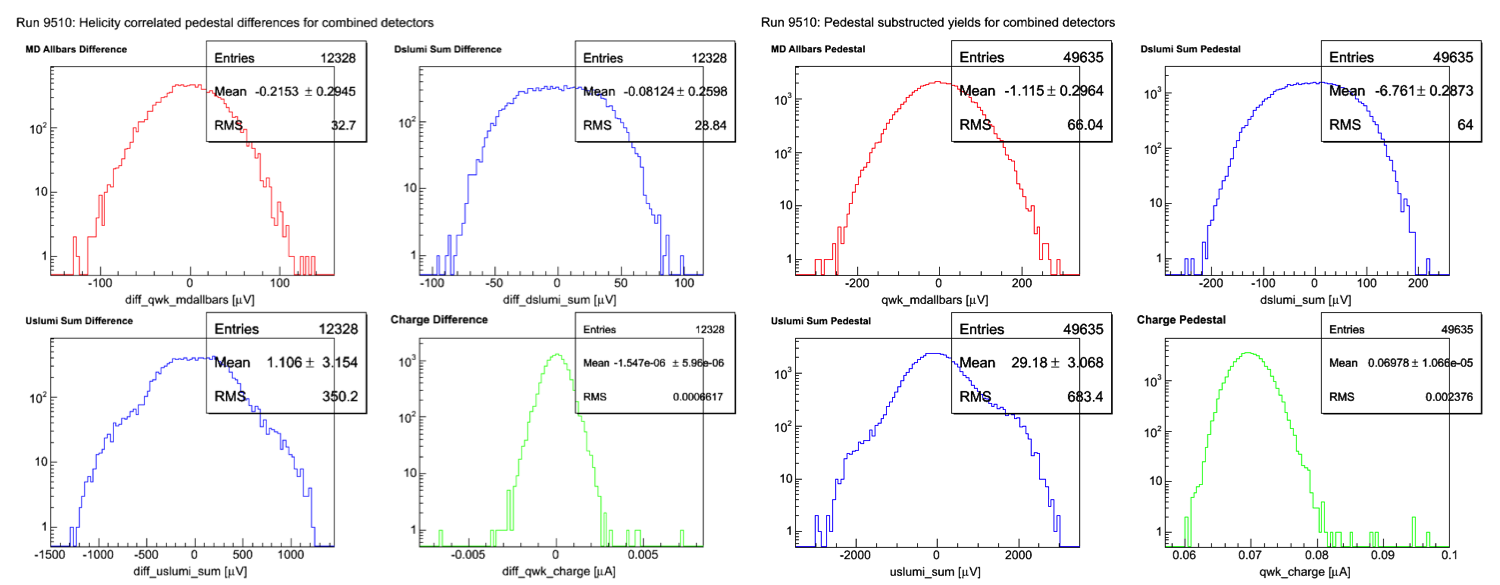
\includegraphics[width=15.0cm]{figures/run}
%	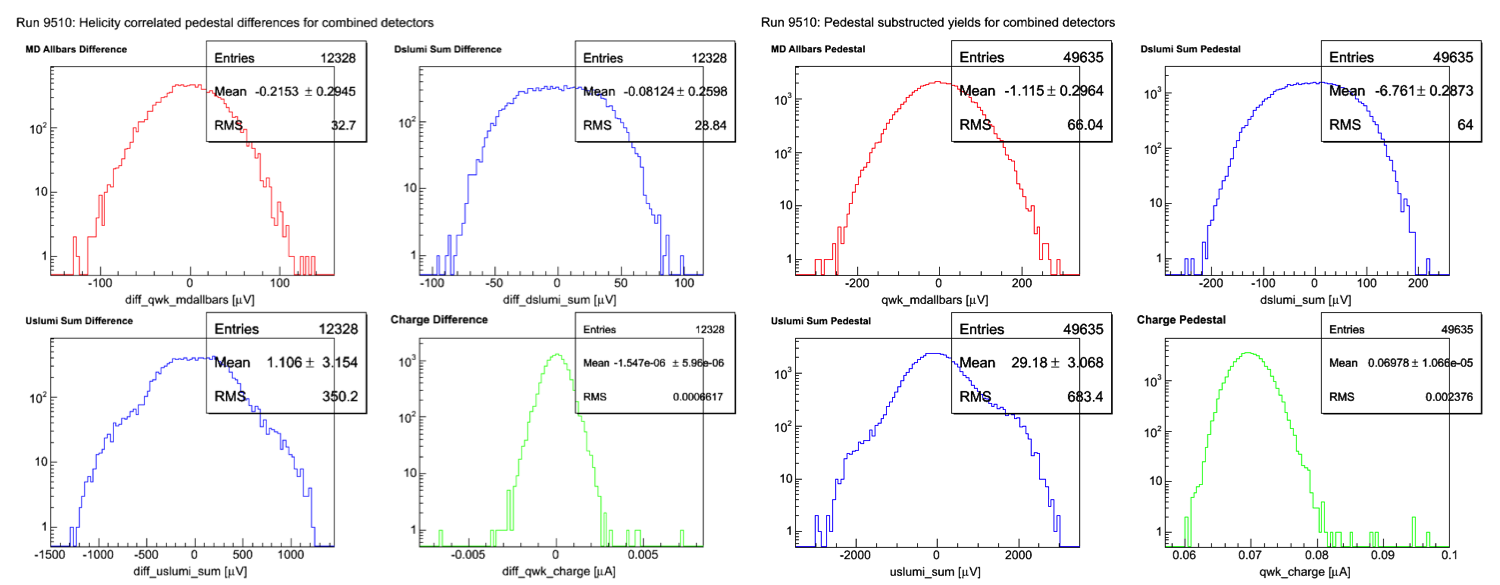
\includegraphics[width=\figSize]{figures/run}
	\end{center}
	\caption
%	[A typical beam off pedestal run distributions from Hel\_Tree and Mps\_Tree.]
	{A typical beam off pedestal run (run\# 9510). Helicity correlated differences for MDAllbars, DSLumiSum, USLumiSum, Charge (clockwise from top left corner) from Hel\_Tree are shown in the left panel. Pedestal subtracted signal for MDAllbars, DSLumiSum, USLumiSum, Charge (clockwise from top left corner) from Mps\_Tree are shown in the right panel.}
	\label{fig:run_hel_tree}
\end{figure}
\end{singlespace}


\subsection{Results}
\label{Results}
The main detectors and luminosity monitors are normalized to the charge monitors so it is important that neither have any evidence of helicity correlated pedestal differences. Helicity correlated differences from Hel\_Tree of a typical 5~minutes pedestal run are shown in Figure~\ref{fig:run_hel_tree}. Even with only 5~minutes of data, no evidence of any helicity correlated pick ups for combined \v{C}erenkov main detector (MDAllbars), downstream luminosity monitor (DSLumiSum), upstream luminosity monitor (USLumiSum), and beam charge monitor (Charge) were seen. 
The channels surveyed during this analysis are 17 MDs, 9 DSLumis, 9 USLumis, and 9 BCMs (details of the variables are described in APPENDIX~\ref{Helicity Corelated Pedestal Analysis 2}, section~\ref{List of Variables}). The individual channels of the MDs, DSLumis, USLumis, and BCMs showed no significant pickup. All these channels were investigated individually for each run and then averaged (error weighted) over a Wien\footnote{Experiment has total 11 Wien period. Double Wien filters were rotated to change the electron beam polarization. This help reducing the false asymmetry.}.
The Wien averaged helicity correlated differences for most important channels for the experiment MDAllbars, DSLumiSum, USLumiSum, and Charge\footnote{Charge = bcm1 + bcm2 for Run 1 and = bcm8 for Run 2.} are shown in Figure~\ref{fig:differencesSum}. 

\begin{singlespace}
\begin{figure}[!h]
	\centering
%	\includegraphics[width=17.5cm]{figures/ScaleHelCorDifffinal_sum_combined_ped_plot}
%	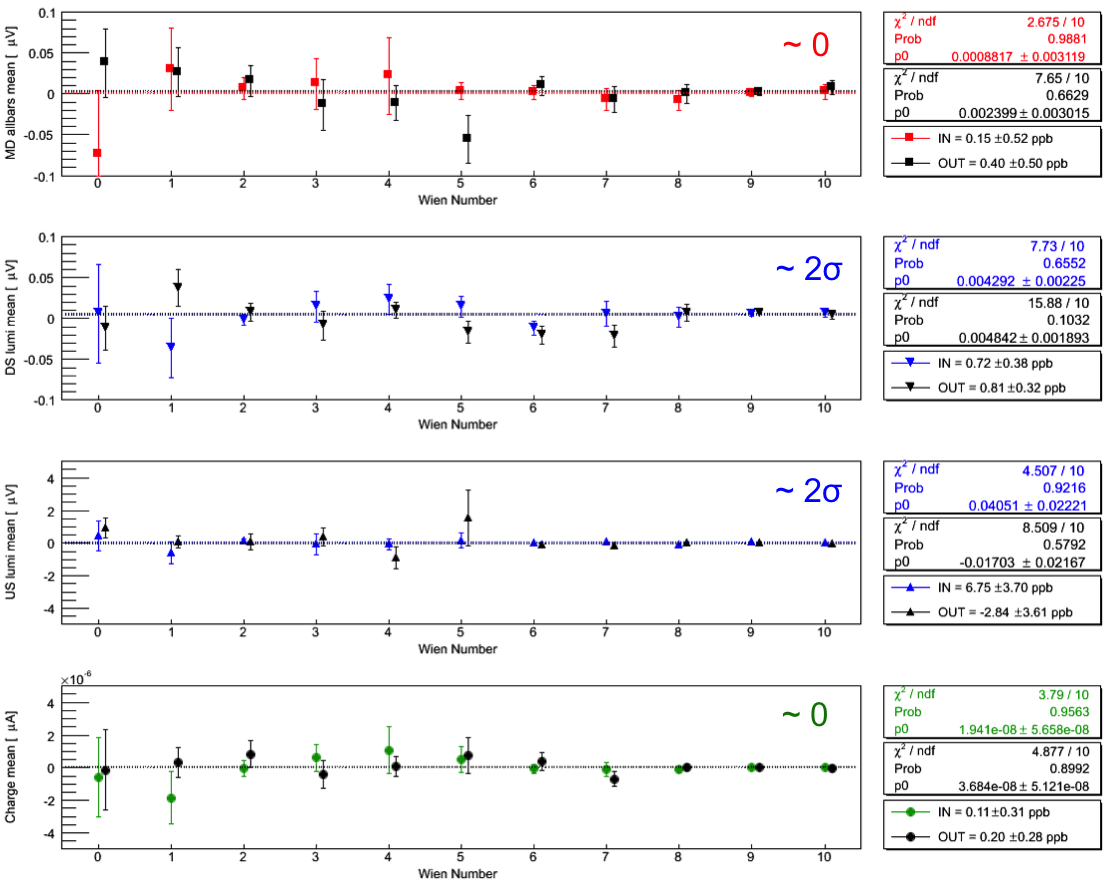
\includegraphics[width=15.0cm]{figures/differencesSum}
	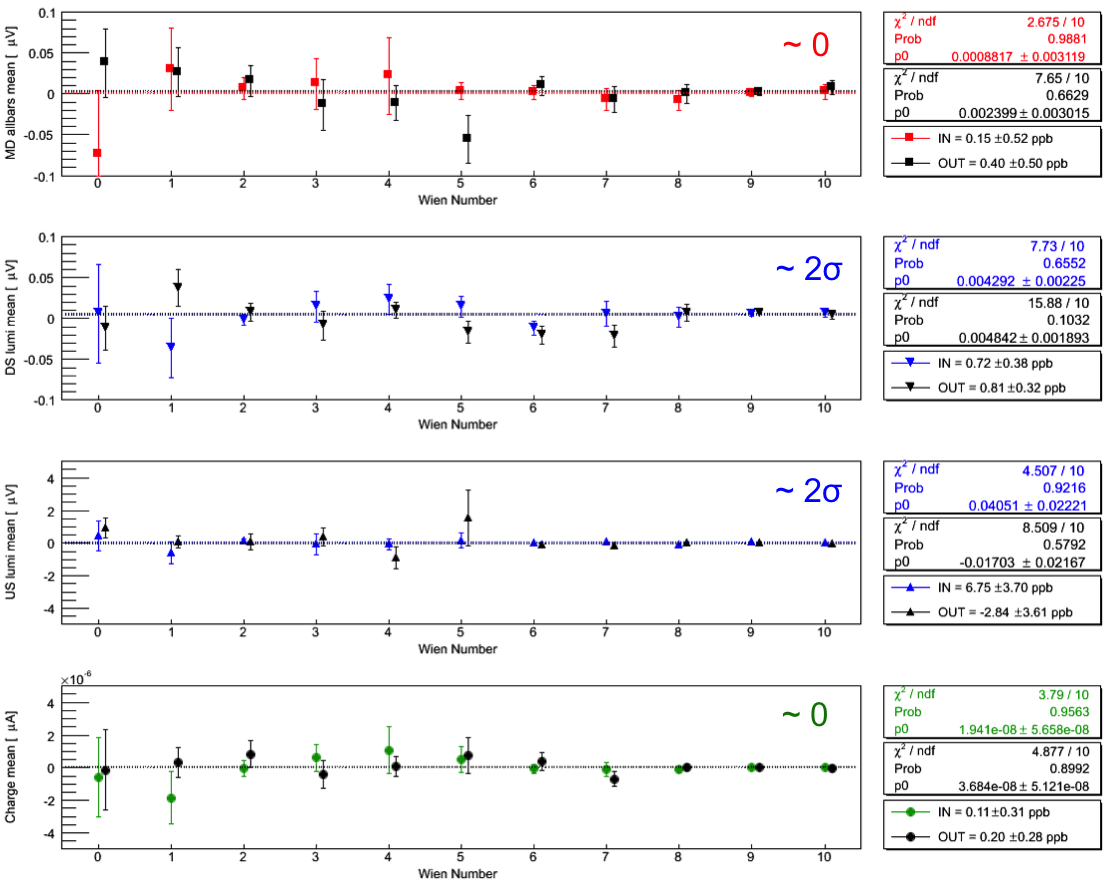
\includegraphics[width=15.0cm]{figures/differencesSum}	
	\caption
%	[The mean of the pedestal differences from Hel\_Tree.]
	{The mean of the pedestal differences from Hel\_Tree for MD allbars, DS lumi, US lumi and Charge are shown. Each data point is averaged over a Wien. Two half wave plate states are shown separately.}
	\label{fig:differencesSum}
\end{figure}
\end{singlespace}

%%----------------------------------------------------%%
\subsubsection{Helicity Correlated Pedestal Signal Pickup}
\label{Helicity Correlated Pedestal Signal Pickup}
The mean of the pedestal differences from Hel\_Tree in Figure~\ref{fig:run_hel_tree} represent the helicity correlated pickup by a device. The surveyed result shows that the average pickup for MD is 0.15~$\pm$~0.52~ppb for insertable half wave plate (IHWP) IN, and 0.40~$\pm$~0.50~ppb for IHWP OUT (shown in Figure~\ref{fig:differencesSum} by colored and black data points, respectively). So helicity correlated pedestal differences have negligible contribution ($\sim$0.2\%) to any false asymmetries in the measured asymmetry. DS Lumi has a similar level of pickup as the MD. US Lumi shows $\sim$7~ppb pickup in worst case scenario which can be improved by using a better pedestal subtraction. BCMs have no pickups for the whole experiment. Overall pickup was much smaller during Run 2 (Wien 6 - 10) compared to Run 1 (Wien 0 - 5), and Run-0 (Wien 0). 

\begin{singlespace}
\begin{figure}[!h]
	\centering
	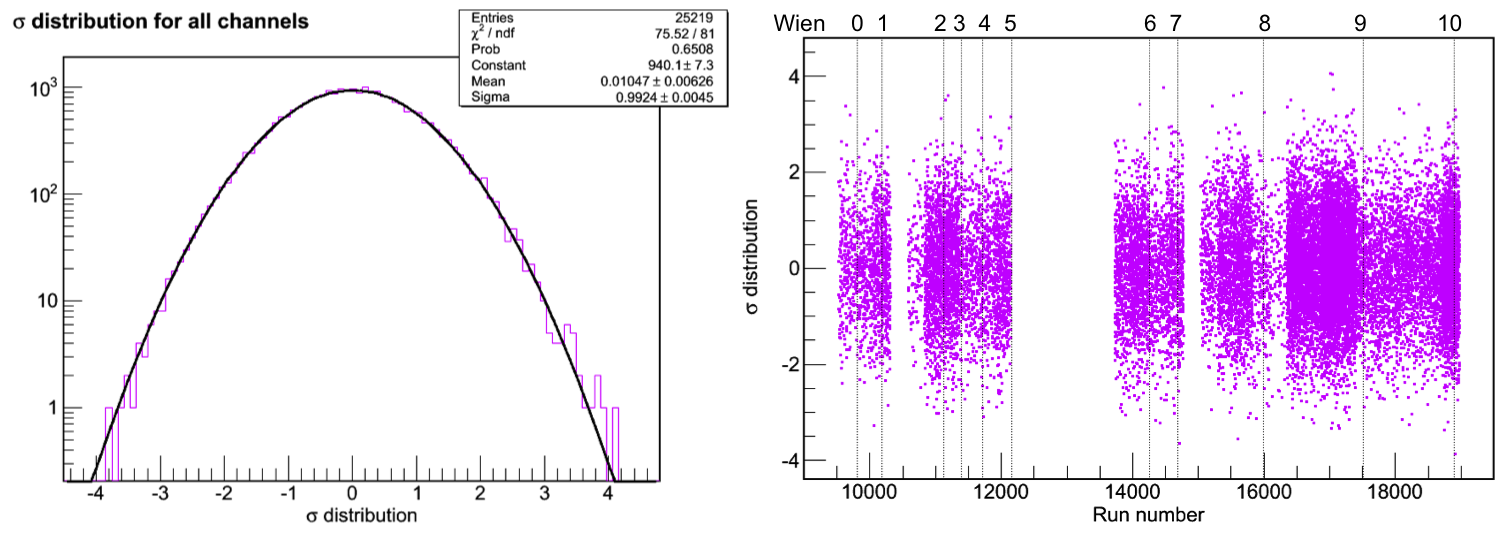
\includegraphics[width=15.0cm]{figures/sigmaDistribution}
	\caption
%	[The pull distribution of helicity correlated pedestal differences.]
	{The pull distribution of helicity correlated pedestal differences for all channels and Wien (left). The data are from the pedestal runs taken during the Q-weak experiment. The black curve in the pull distribution plot is the Gaussian fit. The ostensibly non-zero mean is probably statistical and corresponds to roughly 0.1~$\pm$~0.06~ppb. The pull of helicity correlated pedestal differences vs run number for all the channels are shown (right). The vertical dotted lines represent the Wien periods.}
	\label{fig:sigmaDistribution}
\end{figure}
\end{singlespace}




A pull variable helps to evaluate data points that pull the mean of the distribution and can be defined as 

\begin{equation} \label{equ:calcPedError}
\sigma(ped)_{i,j,k} = \frac{<P>_{i,j,k}}{error_{i,j,k}}
\end{equation}

\noindent
where $<P>$ is the mean helicity correlated pedestal difference and the indices i,j,k denote channel number, run number and IHWP state, respectively.
The distribution of $\sigma(ped)_{i,j,k}$ for each channel and run is shown in Figure~\ref{fig:sigmaDistribution}. 
The distribution of $\sigma(ped)_{i,j,k}$ is Gaussian and the mean is zero for each channel and run. The few $\sigma$ from zero pickup for different detectors are within the statistical fluctuation. 
Mean of the helicity correlated differences for important background detectors (MD9, PMT only, PMT lightguide) were zero within $\sim$1$\sigma$ for each Wien whereas for other background detectors pickups were zero within $\sim$3$\sigma$. Several channels were examined in many pedestal runs, hence it was not unexpected to find a few channels that were non-zero by 3-4$\sigma$ off the mean.
%Because many channels were examined in many pedestal runs, it was of no surprise to find a few that were non-zero by 3-4$\sigma$ off the mean. A pull plot is helpful in evaluating data points that pull the mean of the distribution. Define the pull variable as,

%To summarize:
%\begin{itemize}
%\item No helicity correlated signal pickup within $\sim$2$\sigma$ for combined detectors and averaged over each wien.
%\item Helicity correlated pickup during Q-weak running was consistent with zero for all channels, with a sensitivity at the $\pm$ 1~ppb level for most channels. 
%\item The $\sigma$ distribution is Gaussian and few $\sigma$ from zero pickups for different detectors are within the statistical fluctuation of the distribution.
%\end{itemize}

\begin{singlespace}
\begin{figure}[!h]
	\centering
%	\includegraphics[width=17.5cm]{figures/ScaleHelCorDifffinal_sum_combined_ped_plot}
	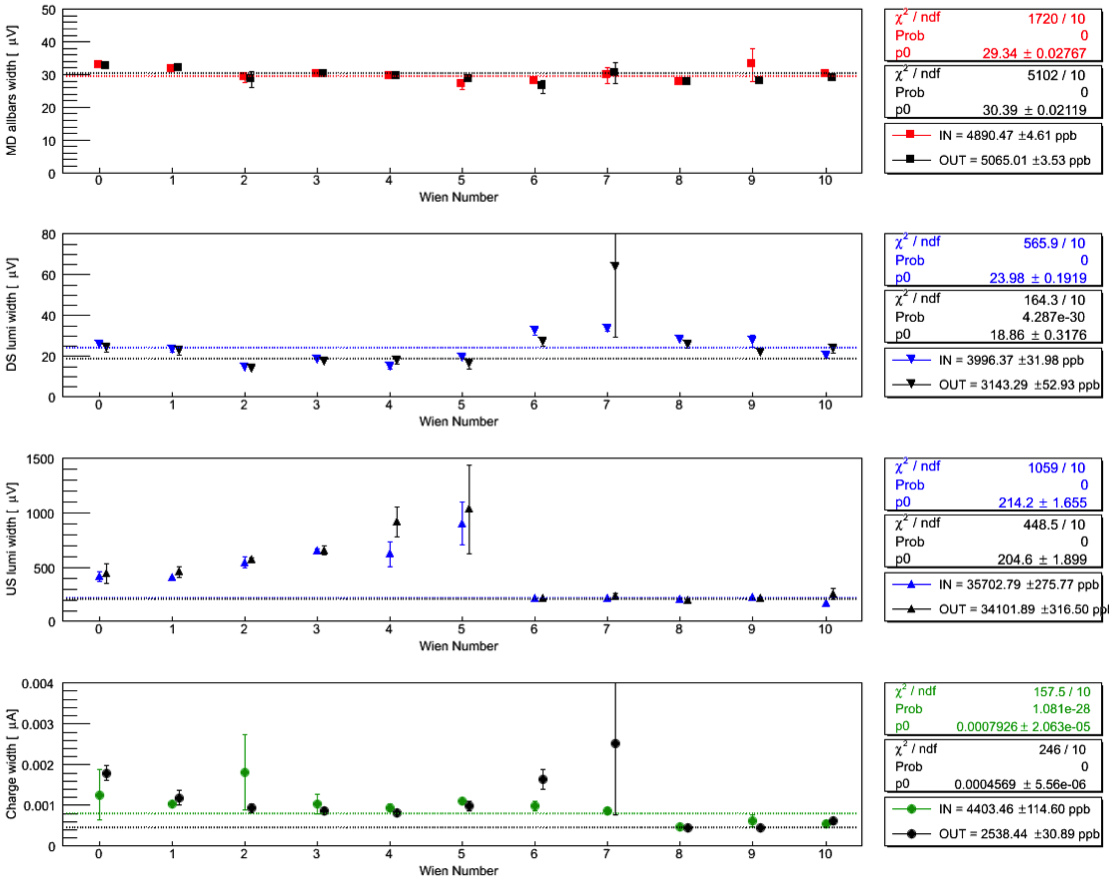
\includegraphics[width=15.0cm]{figures/differencesSumWidth}
	\caption
%	[The width of the pedestal differences from Hel\_Tree.]
	{The width of the pedestal differences from Hel\_Tree for MDAllbars, DSLumiSum, USLumiSum and Charge are shown.}
	\label{fig:differencesSumWidth}
\end{figure}
\end{singlespace}

%%----------------------------------------------------%%
\subsubsection{Helicity Correlated Pedestal Sensitivities}
\label{Helicity Correlated Pedestal Sensitivities}
%\subsection{Detector Resolution}
%\label{Electronic Resolution}
The helicity correlated pedestal difference width from Hel\_Tree represents the sensitivity of a device to the helicity. It also depicts the measure of the electronic noise level for the detectors with low frequency rejection. The Wien averaged helicity correlated differences width for MDAllbars, DSLumiSum, USLumiSum, and Charge are shown in Figure~\ref{fig:differencesSumWidth}. The average noise level of MDAllbars was 25~$\mu$V.
%Width of helicity correlated differences are measure of electronic noise level for our detectors with low frequency rejection.
The MDs and the DSLumis noise levels were acceptable and well behaved throughout the experiment. USLumi electronic noise could have limited the detector's resolution near the end of Run 1, but improved in Run 2 after hardware repairs. Background detectors noise levels were reasonably stable during the experiment.
%(see Figure~\ref{fig: APPENDIX})

%\begin{itemize}
%\item[$\circ$] MDs, DSLumis electronic noise levels acceptable and reasonably stable.
%\item[$\circ$] USLumi noise could have limited that detector's resolution near end of Run 1, but improved in Run 2 after repairs.
%\end{itemize}

\begin{singlespace}
\begin{figure}[!h]
	\centering
	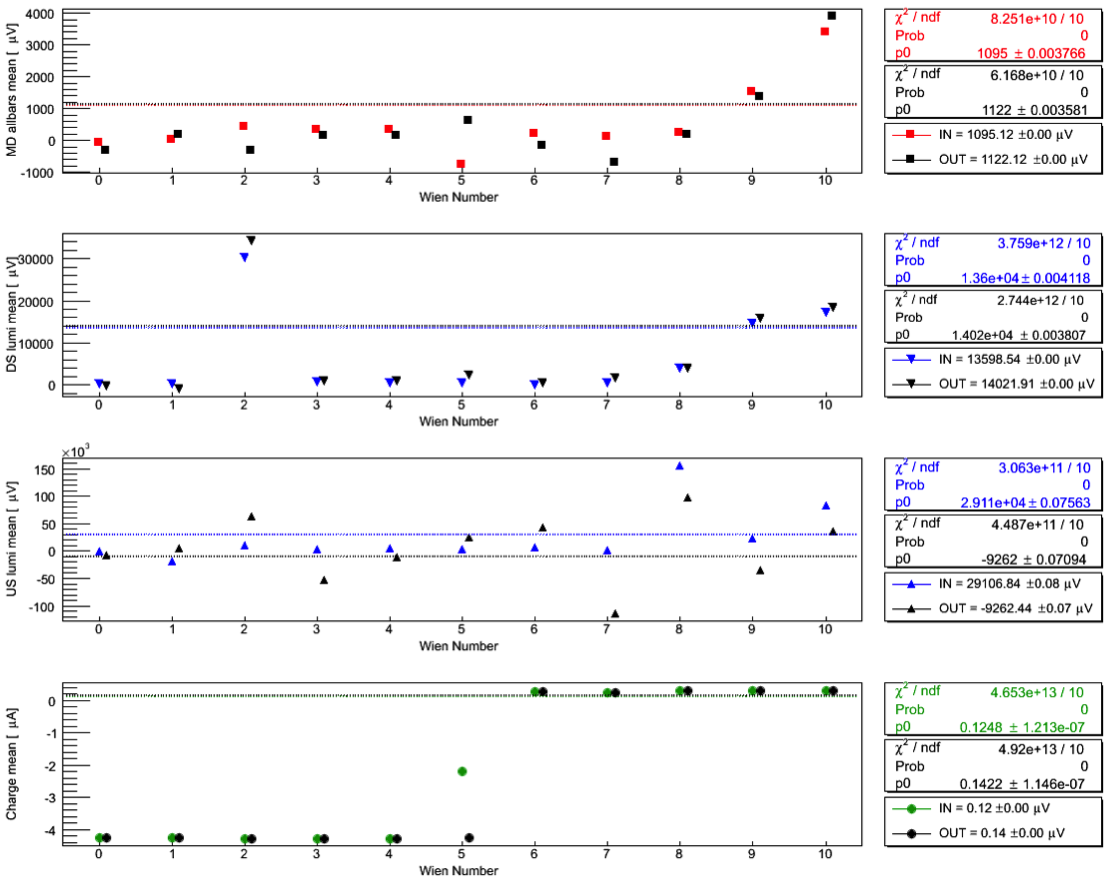
\includegraphics[width=15.0cm]{figures/pedestalSum}
	\caption
%	[The mean of pedestal subtracted signal from Mps\_Tree.]
	{The mean of pedestal subtracted signal from Mps\_Tree for MDAllbars, DSLumiSum, USLumiSum and Charge are shown.}
	\label{fig:pedestalSum}
\end{figure}
\end{singlespace}

%%----------------------------------------------------%%
\subsubsection{Stability of Pedestal Subtracted Signal}
\label{Stability of Pedestal Subtracted Signal}
%\subsection{Mean of Pedestal Subtracted Signal from $Mps\_Tree$}
%\label{Mean of Pedestal Subtracted Signal from $MpsTree$}
%\subsection{Detector Nonlinearity}
%\label{Detector Nonlinearity}
The mean of pedestal subtracted signal from Mps\_Tree represent the relative change in pedestal signal compared to last pedestal. A wrong pedestal for a detector can cause nonlinearity in the detector system. MD pedestal was good to less than a mV (Figure~\ref{fig:pedestalSum}). This results a nonlinearity of $\ll$ 0.1\% for 6~V signals. The detector yields are smaller for Aluminum and N$\rightarrow\Delta$ running compared to normal production running. The signal sizes are $\sim$30-40\% of 6~V. So the nonlinearity for these cases are higher but still $\textless$ 1\%, allowing for smaller yields. DSLumi pedestal was off by at most 34~mV. The resulting nonlinearity would be $\textless$ 1$\%$ assuming 6~V signals. To support Aluminum and N$\rightarrow\Delta$ running, pedestal subtraction should be improved in Wiens 2, 9, 10.  USLumi pedestal was off by 100-150~mV in Wiens 7, 8 and could result a nonlinearity of several percent.
% Resulting nonlinearity would be several percent. %For the transverse N$\rightarrow\Delta$ running discussed in the following chapter the pedestal were matched quite well.


%To summarize:
%\begin{itemize}
%\item[\tiny$\blacksquare$] MD pedestal is good to a few~mV. Resulting nonlinearity would be << 0.1\% for 6~V signals also under control for Aluminum or N-to-Delta running.
%\item[\tiny$\blacksquare$] DSLumi nonlinearity would be < 1\% and several percent for USLumi assuming 6~V signals. To support Aluminum running, etc., pedestal subtraction should be improved for few Wiens.
%\end{itemize}

\begin{singlespace}
\begin{figure}[!h]
	\centering
	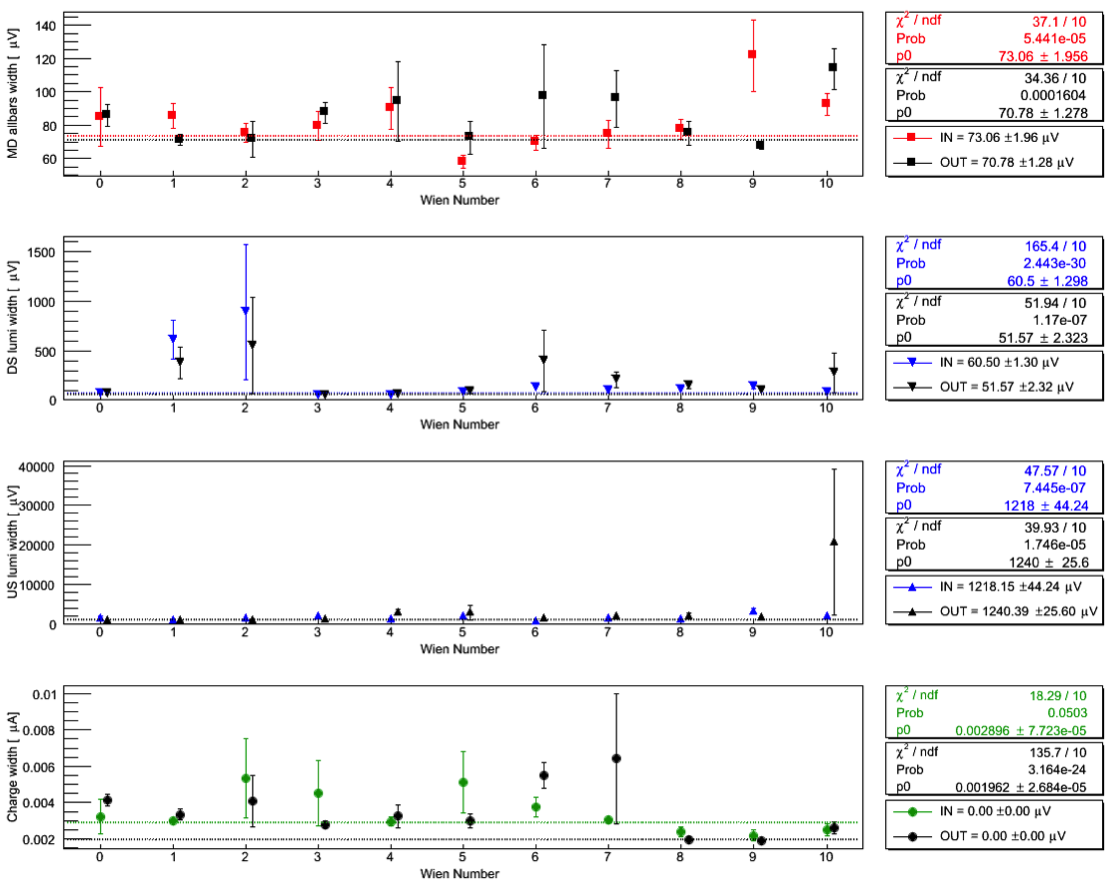
\includegraphics[width=15.0cm]{figures/pedestalSumWidth}
	\caption
%	[The widths of pedestal subtracted signal from Mps\_Tree.]
	{The widths of pedestal subtracted signal from Mps\_Tree for MDAllbars, DSLumiSum, USLumiSum and Charge are shown.}
	\label{fig:pedestalSumWidth}
\end{figure}
\end{singlespace}

%%----------------------------------------------------%%
%\subsection{Width of Pedestal Subtracted Signal from $MpsTree$}
%\label{Width of Pedestal Subtracted Signal from $MpsTree$}
%\subsection{Electronic Noise}
%\label{Electronic Noise}
\subsubsection{Detector Resolution}
\label{Detector Resolution}

The width of pedestal subtracted signal from Mps\_Tree describes the measure of detector resolution. Resolutions for MDs and DSLumis were very good ($\sim$70~$\mu$V) and reasonably stable during the experiment (see Figure~\ref{fig:pedestalSumWidth}). USLumis resolutions were $\sim$15~times worse than MDs and DSLumis but were very stable. The resolutions for charge monitors and background detectors (except PMT LED) were steady throughout the experiment. 

%\begin{itemize}
%\item[\tiny$\square$] MDs, DSLumis, and Charge monitors had very good resolution with reasonably stability.
%\item[\tiny$\square$] USLumis were more noisier, resolution were reasonable but very stable.
%\end{itemize}


\subsection{Summary of Helicity Correlated Pedestal Survey}
\label{Summary of Helicity Correlated Pedestal Survey}
No helicity correlated pickups were seen for most of the detector channels for the entire experiment and were at $\mathcal{O}$(1)~ppb. Electronic noise levels were generally acceptable, though potentially marginal, for the USLumi channels near the end of Run 1 but improved during Run 2. The nonlinearities due to pedestal errors for MDs were extremely small. USLumi also had a nonlinearity of few percent. There is a scope for improvement in USLumi pedestal. The nonlinearity could be very large for low-yield production running on Aluminum and N$\rightarrow\Delta$ but still be under 1\%. Resolutions for all the detectors were reasonably stable. 
%A summary of helicity correlated pedestal survey all the results discussed are shown in Table~\ref{tab:summary}
The helicity correlated pedestal survey results are summarized in Table~\ref{tab:summary}.

\begin{table}[!h]
\begin{center}
  	\caption
%  	[Summary of helicity correlated pedestal survey.]
  	{Summary of helicity correlated pedestal survey.}
  \begin{tabular}{ l | c | c | c | c }
%    \hline
    \noalign{\hrule height 1pt}
    \multirow{2}{*}{Channels}  & False Asymmetry & \multirow{2}{*}{Sensitivity} & Nonlinearity & \multirow{2}{*}{Electronic Noise} \\
              &      [ppb]      &    & [\%] &    \\ 
%    \hline
    \noalign{\hrule height 1pt}
    MDAllbars 	& 0.4 	& 30~$\mu$V     		& $\ll$0.1  		& 73~$\mu$V \\
    DSLumiSum 	& 0.8 	& 24~$\mu$V    		& $<$1.0   		& 61~$\mu$V \\
    USLumiSum 	& 6.8 	& 214~$\mu$V    	& $\sim$1.0 	& 1240~$\mu$V \\
    Charge    	& 0.2 	& 0.0079~$\mu$A 	& $<$0.1   		& 0.0029~$\mu$A \\
%    \hline
    \noalign{\hrule height 1pt}
  	\end{tabular}
  \label{tab:summary}
\end{center}
\end{table}

